%----------------------------------------------------------------------------------------
%	LOCALE
%----------------------------------------------------------------------------------------
\newcommand{\mylocale}{RUS} % Use ENG or RUS

%----------------------------------------------------------------------------------------
%	DOCUMENT TYPE
%----------------------------------------------------------------------------------------
\documentclass{article}

%----------------------------------------------------------------------------------------
%	GENERAL OPTIONS
%----------------------------------------------------------------------------------------
%%%%%%%%%%%%%%%%%%%%%%%%%%%%%%%%%%%%%%%%%
% Lachaise Assignment
% Structure Specification File
% Version 1.0 (26/6/2018)
%
% This template originates from:
% http://www.LaTeXTemplates.com
%
% Authors:
% Marion Lachaise & François Févotte
% Vel (vel@LaTeXTemplates.com)
%
% License:
% CC BY-NC-SA 3.0 (http://creativecommons.org/licenses/by-nc-sa/3.0/)
% 
%%%%%%%%%%%%%%%%%%%%%%%%%%%%%%%%%%%%%%%%%

%----------------------------------------------------------------------------------------
%	PACKAGES AND OTHER DOCUMENT CONFIGURATIONS
%----------------------------------------------------------------------------------------

\usepackage{amsmath,amsfonts,stmaryrd,amssymb} % Math packages
\newcommand{\Lagr}{\mathcal{L}}

\usepackage{enumerate} % Custom item numbers for enumerations

\usepackage[ruled]{algorithm2e} % Algorithms

\usepackage[framemethod=tikz]{mdframed} % Allows defining custom boxed/framed environments

\usepackage{titlesec}

\usepackage{listings} % File listings, with syntax highlighting
\lstset{
	basicstyle=\ttfamily, % Typeset listings in monospace font
}

\usepackage{physics} % Физические обозначения

\usepackage{indentfirst} % Красная строка в первом предложении

\usepackage{appendix} % Приложения

%----------------------------------------------------------------------------------------
%	DOCUMENT MARGINS
%----------------------------------------------------------------------------------------

\usepackage{geometry} % Required for adjusting page dimensions and margins

\geometry{
	paper=a4paper, % Paper size, change to letterpaper for US letter size
	top=2.0cm, % Top margin
	bottom=2.0cm, % Bottom margin
	left=2.0cm, % Left margin
	right=1.5cm, % Right margin
	headheight=14pt, % Header height
	%footskip=1.5cm, % Space from the bottom margin to the baseline of the footer
	%headsep=0.5cm, % Space from the top margin to the baseline of the header
	%showframe, % Uncomment to show how the type block is set on the page
}

%----------------------------------------------------------------------------------------
%	FONTS
%----------------------------------------------------------------------------------------

%\usepackage[utf8]{inputenc} % Required for inputting international characters
%\usepackage[T1]{fontenc} % Output font encoding for international characters
\usepackage[T1,T2A]{fontenc}
\usepackage[utf8]{inputenc}
\usepackage[english,russian]{babel}

\usepackage{XCharter} % Use the XCharter fonts

%----------------------------------------------------------------------------------------
%	COMMAND LINE ENVIRONMENT
%----------------------------------------------------------------------------------------

% Usage:
% \begin{commandline}
%	\begin{verbatim}
%		$ ls
%		
%		Applications	Desktop	...
%	\end{verbatim}
% \end{commandline}

\mdfdefinestyle{commandline}{
	leftmargin=10pt,
	rightmargin=10pt,
	innerleftmargin=15pt,
	middlelinecolor=black!50!white,
	middlelinewidth=2pt,
	frametitlerule=false,
	backgroundcolor=black!5!white,
	frametitle={Command Line},
	frametitlefont={\normalfont\sffamily\color{white}\hspace{-1em}},
	frametitlebackgroundcolor=black!50!white,
	nobreak,
}

% Define a custom environment for command-line snapshots
\newenvironment{commandline}{
	\medskip
	\begin{mdframed}[style=commandline]
}{
	\end{mdframed}
	\medskip
}

%----------------------------------------------------------------------------------------
%	FILE CONTENTS ENVIRONMENT
%----------------------------------------------------------------------------------------

% Usage:
% \begin{file}[optional filename, defaults to "File"]
%	File contents, for example, with a listings environment
% \end{file}

\mdfdefinestyle{file}{
	innertopmargin=1.6\baselineskip,
	innerbottommargin=0.8\baselineskip,
	topline=false, bottomline=false,
	leftline=false, rightline=false,
	leftmargin=2cm,
	rightmargin=2cm,
	singleextra={%
		\draw[fill=black!10!white](P)++(0,-1.2em)rectangle(P-|O);
		\node[anchor=north west]
		at(P-|O){\ttfamily\mdfilename};
		%
		\def\l{3em}
		\draw(O-|P)++(-\l,0)--++(\l,\l)--(P)--(P-|O)--(O)--cycle;
		\draw(O-|P)++(-\l,0)--++(0,\l)--++(\l,0);
	},
	nobreak,
}

% Define a custom environment for file contents
\newenvironment{file}[1][File]{ % Set the default filename to "File"
	\medskip
	\newcommand{\mdfilename}{#1}
	\begin{mdframed}[style=file]
}{
	\end{mdframed}
	\medskip
}

%----------------------------------------------------------------------------------------
%	NUMBERED QUESTIONS ENVIRONMENT
%----------------------------------------------------------------------------------------

% Usage:
% \begin{question}[optional title]
%	Question contents
% \end{question}

\mdfdefinestyle{question}{
	innertopmargin=1.2\baselineskip,
	innerbottommargin=0.8\baselineskip,
	roundcorner=5pt,
	nobreak,
	singleextra={%
		\draw(P-|O)node[xshift=1em,anchor=west,fill=white,draw,rounded corners=5pt]{%
		Вопрос \theQuestion\questionTitle};
	},
}

\newcounter{Question} % Stores the current question number that gets iterated with each new question

% Define a custom environment for numbered questions
\newenvironment{question}[1][\unskip]{
	\bigskip
	\stepcounter{Question}
	\newcommand{\questionTitle}{~#1}
	\begin{mdframed}[style=question]
}{
	\end{mdframed}
	\medskip
}

%----------------------------------------------------------------------------------------
%	WARNING TEXT ENVIRONMENT
%----------------------------------------------------------------------------------------

% Usage:
% \begin{warn}[optional title, defaults to "Warning:"]
%	Contents
% \end{warn}

\mdfdefinestyle{warning}{
	topline=false, bottomline=false,
	leftline=false, rightline=false,
	nobreak,
	singleextra={%
		\draw(P-|O)++(-0.5em,0)node(tmp1){};
		\draw(P-|O)++(0.5em,0)node(tmp2){};
		\fill[black,rotate around={45:(P-|O)}](tmp1)rectangle(tmp2);
		\node at(P-|O){\color{white}\scriptsize\bf !};
		\draw[very thick](P-|O)++(0,-1em)--(O);%--(O-|P);
	}
}

% Define a custom environment for warning text
\newenvironment{warn}[1][Warning:]{ % Set the default warning to "Warning:"
	\medskip
	\begin{mdframed}[style=warning]
		\noindent{\textbf{#1}}
}{
	\end{mdframed}
}

%----------------------------------------------------------------------------------------
%	INFORMATION ENVIRONMENT
%----------------------------------------------------------------------------------------

% Usage:
% \begin{info}[optional title, defaults to "Info:"]
% 	contents
% 	\end{info}

\mdfdefinestyle{info}{%
	topline=false, bottomline=false,
	leftline=false, rightline=false,
	nobreak,
	singleextra={%
		\fill[black](P-|O)circle[radius=0.4em];
		\node at(P-|O){\color{white}\scriptsize\bf i};
		\draw[very thick](P-|O)++(0,-0.8em)--(O);%--(O-|P);
	}
}

% Define a custom environment for information
\newenvironment{info}[1][Информация:]{ % Set the default title to "Info:"
	\medskip
	\begin{mdframed}[style=info]
		\noindent{\textbf{#1}}
}{
	\end{mdframed}
}

%----------------------------------------------------------------------------------------
%	IMAGES
%----------------------------------------------------------------------------------------

\usepackage{graphicx}
\graphicspath{{images/}}
\DeclareGraphicsExtensions{.pdf,.png,.jpg}

%----------------------------------------------------------------------------------------
%	TITLE AND OTHER OPTIONS
%----------------------------------------------------------------------------------------
\ifthenelse{\equal{\mylocale}{ENG}}
{
    %----------------------------------------------------------------------------------------
%	COMMAND LINE ENVIRONMENT
%----------------------------------------------------------------------------------------

% Usage:
% \begin{commandline}
%	\begin{verbatim}
%		$ ls
%		
%		Applications	Desktop	...
%	\end{verbatim}
% \end{commandline}

\mdfdefinestyle{commandline}{
	leftmargin=10pt,
	rightmargin=10pt,
	innerleftmargin=15pt,
	middlelinecolor=black!50!white,
	middlelinewidth=2pt,
	frametitlerule=false,
	backgroundcolor=black!5!white,
	frametitle={Maple Code},
	frametitlefont={\normalfont\sffamily\color{white}\hspace{-1em}},
	frametitlebackgroundcolor=black!50!white,
	nobreak,
}

% Define a custom environment for command-line snapshots
\newenvironment{commandline}{
	\medskip
	\begin{mdframed}[style=commandline]
}{
	\end{mdframed}
	\medskip
}

%----------------------------------------------------------------------------------------
%	FILE CONTENTS ENVIRONMENT
%----------------------------------------------------------------------------------------

% Usage:
% \begin{file}[optional filename, defaults to "File"]
%	File contents, for example, with a listings environment
% \end{file}

\mdfdefinestyle{file}{
	innertopmargin=1.6\baselineskip,
	innerbottommargin=0.8\baselineskip,
	topline=false, bottomline=false,
	leftline=false, rightline=false,
	leftmargin=2cm,
	rightmargin=2cm,
	singleextra={%
		\draw[fill=black!10!white](P)++(0,-1.2em)rectangle(P-|O);
		\node[anchor=north west]
		at(P-|O){\ttfamily\mdfilename};
		%
		\def\l{3em}
		\draw(O-|P)++(-\l,0)--++(\l,\l)--(P)--(P-|O)--(O)--cycle;
		\draw(O-|P)++(-\l,0)--++(0,\l)--++(\l,0);
	},
	nobreak,
}

% Define a custom environment for file contents
\newenvironment{file}[1][File]{ % Set the default filename to "File"
	\medskip
	\newcommand{\mdfilename}{#1}
	\begin{mdframed}[style=file]
}{
	\end{mdframed}
	\medskip
}

%----------------------------------------------------------------------------------------
%	NUMBERED QUESTIONS ENVIRONMENT
%----------------------------------------------------------------------------------------

% Usage:
% \begin{question}[optional title]
%	Question contents
% \end{question}

\mdfdefinestyle{question}{
	innertopmargin=1.2\baselineskip,
	innerbottommargin=0.8\baselineskip,
	roundcorner=5pt,
	nobreak,
	singleextra={%
		\draw(P-|O)node[xshift=1em,anchor=west,fill=white,draw,rounded corners=5pt]{%
		Question \theQuestion\questionTitle};
	},
}

\newcounter{Question} % Stores the current question number that gets iterated with each new question

% Define a custom environment for numbered questions
\newenvironment{question}[1][\unskip]{
	\bigskip
	\stepcounter{Question}
	\newcommand{\questionTitle}{~#1}
	\begin{mdframed}[style=question]
}{
	\end{mdframed}
	\medskip
}

%----------------------------------------------------------------------------------------
%	WARNING TEXT ENVIRONMENT
%----------------------------------------------------------------------------------------

% Usage:
% \begin{warn}[optional title, defaults to "Warning:"]
%	Contents
% \end{warn}

\mdfdefinestyle{warning}{
	topline=false, bottomline=false,
	leftline=false, rightline=false,
	nobreak,
	singleextra={%
		\draw(P-|O)++(-0.5em,0)node(tmp1){};
		\draw(P-|O)++(0.5em,0)node(tmp2){};
		\fill[black,rotate around={45:(P-|O)}](tmp1)rectangle(tmp2);
		\node at(P-|O){\color{white}\scriptsize\bf !};
		\draw[very thick](P-|O)++(0,-1em)--(O);%--(O-|P);
	}
}

% Define a custom environment for warning text
\newenvironment{warn}[1][Warning:]{ % Set the default warning to "Warning:"
	\medskip
	\begin{mdframed}[style=warning]
		\noindent{\textbf{#1}}
}{
	\end{mdframed}
}

%----------------------------------------------------------------------------------------
%	INFORMATION ENVIRONMENT
%----------------------------------------------------------------------------------------

% Usage:
% \begin{info}[optional title, defaults to "Info:"]
% 	contents
% 	\end{info}

\mdfdefinestyle{info}{%
	topline=false, bottomline=false,
	leftline=false, rightline=false,
	nobreak,
	singleextra={%
		\fill[black](P-|O)circle[radius=0.4em];
		\node at(P-|O){\color{white}\scriptsize\bf i};
		\draw[very thick](P-|O)++(0,-0.8em)--(O);%--(O-|P);
	}
}

% Define a custom environment for information
\newenvironment{info}[1][Info:]{ % Set the default title to "Info:"
	\medskip
	\begin{mdframed}[style=info]
		\noindent{\textbf{#1}}
}{
	\end{mdframed}
}
    \title{\textbf{Ritz Method}} % Title

\author[1]{Nikolay Zhivotenko} % Author name, email address, university department name(s)

\date{\small \mydate} % Date

\affil[1]{\small M.Sc., Department of Rocket and Space Composite Structures, Bauman MSTU}
\affil[1]{\small B.Sc., Department of Solid State Physics, VorSTU}
\affil[1]{\small \texttt{niko.zvt@gmail.com}}
}{}

\ifthenelse{\equal{\mylocale}{RUS}}
{
    %----------------------------------------------------------------------------------------
%	COMMAND LINE ENVIRONMENT
%----------------------------------------------------------------------------------------

% Usage:
% \begin{commandline}
%	\begin{verbatim}
%		$ ls
%		
%		Applications	Desktop	...
%	\end{verbatim}
% \end{commandline}

\mdfdefinestyle{commandline}{
	leftmargin=10pt,
	rightmargin=10pt,
	innerleftmargin=15pt,
	middlelinecolor=black!50!white,
	middlelinewidth=2pt,
	frametitlerule=false,
	backgroundcolor=black!5!white,
	frametitle={Maple Code},
	frametitlefont={\normalfont\sffamily\color{white}\hspace{-1em}},
	frametitlebackgroundcolor=black!50!white,
	nobreak,
}

% Define a custom environment for command-line snapshots
\newenvironment{commandline}{
	\medskip
	\begin{mdframed}[style=commandline]
}{
	\end{mdframed}
	\medskip
}

%----------------------------------------------------------------------------------------
%	FILE CONTENTS ENVIRONMENT
%----------------------------------------------------------------------------------------

% Usage:
% \begin{file}[optional filename, defaults to "File"]
%	File contents, for example, with a listings environment
% \end{file}

\mdfdefinestyle{file}{
	innertopmargin=1.6\baselineskip,
	innerbottommargin=0.8\baselineskip,
	topline=false, bottomline=false,
	leftline=false, rightline=false,
	leftmargin=2cm,
	rightmargin=2cm,
	singleextra={%
		\draw[fill=black!10!white](P)++(0,-1.2em)rectangle(P-|O);
		\node[anchor=north west]
		at(P-|O){\ttfamily\mdfilename};
		%
		\def\l{3em}
		\draw(O-|P)++(-\l,0)--++(\l,\l)--(P)--(P-|O)--(O)--cycle;
		\draw(O-|P)++(-\l,0)--++(0,\l)--++(\l,0);
	},
	nobreak,
}

% Define a custom environment for file contents
\newenvironment{file}[1][File]{ % Set the default filename to "File"
	\medskip
	\newcommand{\mdfilename}{#1}
	\begin{mdframed}[style=file]
}{
	\end{mdframed}
	\medskip
}

%----------------------------------------------------------------------------------------
%	NUMBERED QUESTIONS ENVIRONMENT
%----------------------------------------------------------------------------------------

% Usage:
% \begin{question}[optional title]
%	Question contents
% \end{question}

\mdfdefinestyle{question}{
	innertopmargin=1.2\baselineskip,
	innerbottommargin=0.8\baselineskip,
	roundcorner=5pt,
	nobreak,
	singleextra={%
		\draw(P-|O)node[xshift=1em,anchor=west,fill=white,draw,rounded corners=5pt]{%
		Вопрос \theQuestion\questionTitle};
	},
}

\newcounter{Question} % Stores the current question number that gets iterated with each new question

% Define a custom environment for numbered questions
\newenvironment{question}[1][\unskip]{
	\bigskip
	\stepcounter{Question}
	\newcommand{\questionTitle}{~#1}
	\begin{mdframed}[style=question]
}{
	\end{mdframed}
	\medskip
}

%----------------------------------------------------------------------------------------
%	WARNING TEXT ENVIRONMENT
%----------------------------------------------------------------------------------------

% Usage:
% \begin{warn}[optional title, defaults to "Warning:"]
%	Contents
% \end{warn}

\mdfdefinestyle{warning}{
	topline=false, bottomline=false,
	leftline=false, rightline=false,
	nobreak,
	singleextra={%
		\draw(P-|O)++(-0.5em,0)node(tmp1){};
		\draw(P-|O)++(0.5em,0)node(tmp2){};
		\fill[black,rotate around={45:(P-|O)}](tmp1)rectangle(tmp2);
		\node at(P-|O){\color{white}\scriptsize\bf !};
		\draw[very thick](P-|O)++(0,-1em)--(O);%--(O-|P);
	}
}

% Define a custom environment for warning text
\newenvironment{warn}[1][Warning:]{ % Set the default warning to "Warning:"
	\medskip
	\begin{mdframed}[style=warning]
		\noindent{\textbf{#1}}
}{
	\end{mdframed}
}

%----------------------------------------------------------------------------------------
%	INFORMATION ENVIRONMENT
%----------------------------------------------------------------------------------------

% Usage:
% \begin{info}[optional title, defaults to "Info:"]
% 	contents
% 	\end{info}

\mdfdefinestyle{info}{%
	topline=false, bottomline=false,
	leftline=false, rightline=false,
	nobreak,
	singleextra={%
		\fill[black](P-|O)circle[radius=0.4em];
		\node at(P-|O){\color{white}\scriptsize\bf i};
		\draw[very thick](P-|O)++(0,-0.8em)--(O);%--(O-|P);
	}
}

% Define a custom environment for information
\newenvironment{info}[1][Информация:]{ % Set the default title to "Info:"
	\medskip
	\begin{mdframed}[style=info]
		\noindent{\textbf{#1}}
}{
	\end{mdframed}
}
    \title{\textbf{Метод конечных элементов}} % Название

\author[1]{Николай Животенко} % Автор, регалии и e-mail

\date{\small \mydate} % Дата

\affil[1]{\small M.Sc., каф. Ракетно-космических композитных конструкций, МГТУ им. Н. Э. Баумана}
\affil[1]{\small B.Sc., каф. Физики твёрдого тела, Воронежский Государственный Технический Университет}
\affil[1]{\small \texttt{niko.zvt@gmail.com}}
}{}

\normalsize

%----------------------------------------------------------------------------------------
%	DOCUMENT
%----------------------------------------------------------------------------------------
\begin{document}

    % Print text
    \maketitle 

    % Print text
    \ifthenelse{\equal{\mylocale}{ENG}} 
    {
        %----------------------------------------------------------------------------------------
%	Introduction
%----------------------------------------------------------------------------------------

\section*{Introduction}

\begin{info}
    Calculus of variations is a mathematical discipline dedicated to finding the extreme (largest and smallest) values of functionals.
    Functionals are variables that depend on the choice of one or more functions.
    The calculus of variations is a natural development of the Chapter of mathematical analysis devoted to the problem of finding extremums of functions.
    The origin and development of the calculus of variations are closely related to the problems of mechanics, physics, and other technical sciences.
\end{info}

Even in ancient times, the first variational problems related to the category of isoperimetric problems appeared -- for example, the Dido problem. The first variational principle formulated by Heron of Alexandria for the trajectories of reflected light beams in "Catoptrica" (I century A.D.). In medieval Europe isoperimetric tasks engaged Sacrobosco (XIII century), and Bradwarden (XIV century). After the development of analysis, new types of variational problems, mostly of a mechanical nature. Newton in "Mathematical principles of natural philosophy" \; (1687) solves the problem: find the shape of the body of rotation that provides the least resistance when moving in a gas or liquid at a given size. An important historical problem that gave impetus to the development of the modern version of the calculus of variations was the brachistochrone problem (1696). Its rapid solution by several mathematicians showed the huge possibilities of new methods. Among other tasks, it is worth noting the determination of the shape of the chain line, that is, the shape of the equilibrium of a heavy homogeneous thread (1690). General methods for solving variational problems did not yet exist at this time, each problem was solved with the help of ingenious and not always perfect geometric reasoning.

Leonhard Euler and Joseph Lagrange made crucial contributions to the development of the calculus of variations. Euler wrote the first systematic exposition of the calculus of variations and the term itself (1766). Joseph Lagrange independently obtained many fundamental results and introduced the concept of variation (since 1755). At this stage, the Euler-Lagrange equations were derived.

Methods of the calculus of variations are widely used in various fields of mathematics. For example, in differential geometry, they are used to search for geodesic lines and minimal surfaces. In physics, the variational method is one of the most powerful tools for obtaining equations of motion for both discrete and distributed systems, including physical fields. The methods of the calculus of variations are also applicable in statics.

There are two main types of methods for solving variational problems. The first type includes methods that reduce the original problem to solving differential equations. The alternative is the so-called direct methods. These methods in one way or another solve the original problem of finding a function in a given class that would deliver an extreme value to a given functional. One of the most popular methods in this class is the Ritz method.

%----------------------------------------------------------------------------------------
%	CHAPTER 1
%----------------------------------------------------------------------------------------

\newpage

\section{Calculus of variations}

\subsection{Concept of functional}

In the course of higher mathematics, the concept of a function was introduced. If some number $x$ from the region $D$ is put into correspondence by a specific rule or law, the number of $u$, then we say that set function $u=f(x)$. The region $D$ is called the domain of the function $f(x)$.

If the function $f(x)$ corresponds to the number $J$ according to a certain rule or law, then it is said that the functional $J = \Phi[f(x)]$ or $J = \Phi[u]$ is given. An example of a functional can be a certain integral of the function $f(x)$ or of some expression that depends on $f(x)$,

\begin{displaymath}
	\Phi[f(x)] = \int_{a}^{b} f(x) \; dx \; \Leftrightarrow \; \Phi[u] = \int_{a}^{b} u \; dx,
\end{displaymath}

\begin{displaymath}
	\Phi[f(x)] = \int_{a}^{b} [f''(x) + p(x)f'(x) + q(x)f(x)] \;  dx \; \Leftrightarrow \; \Phi[u] = \int_{a}^{b} [u'' + p(x)u' + q(x)u] \;  dx. 
\end{displaymath}

If now the function $u = f(x, y)$ is put in accordance with a certain rule or law again the function $v = g(u)$, then we say that the operator $v = L(u)$ or $v = Lu$ is given. Examples of differential operators are:

\begin{displaymath}
	Lu = u'' + p(x,y)u' + q(x,y)u,
\end{displaymath}

\begin{displaymath}
    Lu = \frac{\partial^2 u}{\partial x^2} + \frac{\partial^2 u}{\partial y^2}.
\end{displaymath}

Let's give a stricter definition of the functional. Let $A$ be a set of elements of arbitrary nature, and let each element of $u \in A$ correspond to one and only one number $J = \Phi[u]$. In this case, we say that the set $A$ has the functional $\Phi[u]$. The set $A$ is called the domain of the functional definition $\Phi[u]$ and is denoted by $D(J)$; the number $J$ is called the value of the functional $\Phi[u]$ on the $u$ element. A functional $\Phi[u]$ is called real if all its values are real. A functional $\Phi[u]$ is called linear if its domain of definition is a linear set and if

\begin{displaymath}
    \Phi[\alpha u + \beta w] = \alpha \cdot \Phi[u] + \beta \cdot \Phi[w],
\end{displaymath}

\begin{displaymath}
	\alpha, \beta = const, w \in A.
\end{displaymath}

%------------------------------------------------

\subsection{The problems leading to the extremum of the functional}




























    }{
        %----------------------------------------------------------------------------------------
%	ВВЕДЕНИЕ
%----------------------------------------------------------------------------------------
\section*{Введение} % Ненумерованная секция

\begin{info} % Информационный блок
	Вариационное исчисление -- математическая дисциплина, посвящённая отысканию экстремальных (наибольших и наименьших) значений функционалов -- переменных величин, зависящих от выбора одной или нескольких функций. Вариационное исчисление является естественным развитием той главы математического анализа, которая посвящена задаче отыскания экстремумов функций. Возникновение и развитие вариационного исчисления тесно связано с задачами механики, физики и других технических наук.
\end{info}

Ещё в античные времена появились первые вариационные проблемы, относящиеся к категории изопериметрических задач -- например, задача Дидоны. Первый вариационный принцип сформулировал Герон Александрийский для траекторий отражённых световых лучей в работе «Катоптрика» (I в. н.э.). В средневековой Европе изопериметрическими задачами занимались И. Сакробоско (XIII в.) и Т. Брадвардин (XIV в.). После разработки анализа появились новые типы вариационных задач, в основном механического характера. Ньютон в «Математических началах натуральной философии» (1687 г.) решает задачу: найти форму тела вращения, обеспечивающую наименьшее сопротивление при движении в газе или жидкости при заданных размерах. Важной исторической задачей, давшей толчок к развитию современного варианта вариационного исчисления, стала задача о брахистохроне (1696 г.). Её быстрое решение сразу несколькими математиками показало огромные возможности новых методов. Среди других задач стоит отметить определение формы цепной линии, то есть формы равновесия тяжёлой однородной нити (1690 г.). Общих методов решения вариационных задач в этот период ещё не существовало, каждая задача решалась с помощью остроумных и не всегда безупречных геометрических рассуждений.

Решающий вклад в развитие вариационного исчисления внесли Леонард Эйлер и Жозеф Лагранж. Эйлеру принадлежит первое систематическое изложение вариационного исчисления и сам термин (1766 г.). Лагранж независимо получил многие основополагающие результаты и ввёл понятие вариации (с 1755 г.). На этом этапе были выведены уравнения Эйлера--Лагранжа.

Методы вариационного исчисления широко применяются в различных областях математики. Например, в дифференциальной геометрии с их помощью ищут геодезические линии и минимальные поверхности. В физике вариационный метод -- одно из мощнейших орудий получения уравнений движения, как для дискретных, так и для распределённых систем, в том числе и для физических полей. Методы вариационного исчисления применимы и в статике.

Выделяют два основных типа методов решения вариационных задач. К первому типу относятся методы, сводящие исходную задачу к решению дифференциальных уравнений. Альтернативой являются так называемые прямые методы. Эти методы тем или иным способом решают исходную задачу по поиску функции в заданном классе, которая доставляла бы экстремальное значение заданному функционалу. Один из самых популярных методов этого класса — метод Ритца.

%----------------------------------------------------------------------------------------
%	ГЛАВА 1
%----------------------------------------------------------------------------------------

\newpage

\section{Вариационное исчисление}

\subsection{Понятие функционала}

В курсе высшей математики вводилось понятие функции. Если некоторому числу $x$ из области $D$ ставится в соответствие по определённому правилу или закону число $u$, то говорят, 
что задана функция $u=f(x)$. Область $D$ называют областью определения функции $f(x)$.

Если же функции $f(x)$ ставится в соответствие по определённому правилу или закону число $J$, то говорят, что задан функционал $J = \Phi[f(x)]$ или 
$J = \Phi[u]$. Примером функционала может быть определённый интеграл от функции $f(x)$ или от некоторого выражения, зависящего от $f(x)$,

\begin{displaymath}
	\Phi[f(x)] = \int_{a}^{b} f(x) \; dx \; \Leftrightarrow \; \Phi[u] = \int_{a}^{b} u \; dx,
\end{displaymath}

\begin{displaymath}
	\Phi[f(x)] = \int_{a}^{b} [f''(x) + p(x)f'(x) + q(x)f(x)] \;  dx \; \Leftrightarrow \; \Phi[u] = \int_{a}^{b} [u'' + p(x)u' + q(x)u] \;  dx. 
\end{displaymath}

Если теперь функции $u = f(x, y)$ ставится в соответствие по определённому правилу или закону вновь функция $v = g(u)$, то говорят, что задан оператор $v = L(u)$ или $v = Lu$. Примерами дифференциальных операторов могут служить:

\begin{displaymath}
	Lu = u'' + p(x,y)u' + q(x,y)u,
\end{displaymath}

\begin{displaymath}
    Lu = \frac{\partial^2 u}{\partial x^2} + \frac{\partial^2 u}{\partial y^2}.
\end{displaymath}

Дадим более строгое определение функционала. Пусть $A$ -- множество элементов произвольной природы, и пусть каждому элементу $u \in A$ приведено в соответствие одно и только одно число $J = \Phi[u]$. В этом случае говорят, что на множестве $A$ задан функционал $\Phi[u]$. Множество $A$ называется областью определения функционала $\Phi[u]$ и обозначается через $D(J)$; число $J$ называется значением функционала $\Phi[u]$ на элементе $u$. Функционал $\Phi[u]$ называется вещественным, если все его значения вещественны. Функционал $\Phi[u]$ называется линейным, если его область определения есть линейное множество и если

\begin{displaymath}
    \Phi[\alpha u + \beta w] = \alpha \cdot \Phi[u] + \beta \cdot \Phi[w],
\end{displaymath}

\begin{displaymath}
	\alpha, \beta = const, w \in A.
\end{displaymath}

%------------------------------------------------

\subsection{Задачи, приводящие к экстремуму функционала}

Зарождение вариационного исчисления относят обычно к 1696 году, когда И. Бернулли поставил так называемую задачу о брахистохроне: определить форму кривой, лежащей в вертикальной плоскости, по которой тяжёлая материальная точка, двигаясь под действием только одной силы тяжести и не имеющая начальной скорости, перейдёт из верхнего положения $A$ в нижнее положение $B$ за минимум времени, рисунок \ref{img_brachistochrone}. Эта задача сводится к отысканию исходной функции $y = f(x)$ -- брахистохроны.

\begin{figure}[!ht]
\center{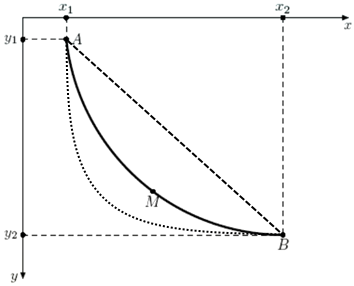
\includegraphics[height=7cm]{images/Brachistochrone_Curve.png}}
\caption{Задача о брахистохроне}
\label{img_brachistochrone}
\end{figure}

Пусть уравнение кривой $AB$ есть $y = f(x)$. Рассмотрим некоторый момент времени $t$, и пусть в этот момент движущаяся точка находится на расстоянии $y$ от оси $x$. Направим ось ординат вниз и сопоставим начальной точке нулевое значение ординаты. Из закона сохранения энергии для материальной точки имеем

\begin{displaymath}
    \frac{m\upsilon^2}{2} = mgy.
\end{displaymath}

Тогда $\upsilon = \sqrt{2gy}$ , где $\upsilon$ -- скорость движущейся точки, $g$ -- ускорение свободного падения, a $y$ -- ордината точки. В то же время:

\begin{displaymath}
    \upsilon = \frac{dS}{dt} = \sqrt{1 + (y')^2} \frac{dx}{dt},
\end{displaymath}

\noindent отсюда следует, что

\begin{displaymath}
    dt = \sqrt{\frac{1 + (y')^2}{2gy}}dx,
\end{displaymath}

\noindent Обозначим через $T$ время, в течение которого материальная точка достигает точки $B$. Интегрируя, находим

\begin{displaymath}
    T = \frac{1}{\sqrt{2g}} \int_{A}^{B} \sqrt{\frac{1 + (y')^2}{y}} \; dx.
\end{displaymath}

Задача сводится к следующему: надо найти функцию $y = f(x)$, удовлетворяющую условию $f(A) = 0$, $f(B) = C$ и сообщающую интегралу наименьшее значение. Условия означают, что искомая кривая должна проходить через заданные точки $A$ и $B$. Такого типа условия принято называть граничными, или краевыми, так как они относятся к концам промежутка, на котором должна быть определена искомая функция.

\begin{info}
	Данная задача относится к ветви математического анализа, называемой вариационным исчислением. Примером применения кривой в виде брахистохроны служит образующая цилиндрических поверхностей, используемых на детских площадках, в аттракционах для спуска с возвышения, на трамплинах.
\end{info}

%------------------------------------------------

\subsection{Первая вариация функционала}

Задача вариационного исчисления состоит в следующем: дан функционал $\Phi[u]$ с областью определения $D(\Phi[u])$; требуется найти элемент $u_{0} \in D(\Phi[u])$,
 сообщающий функционалу либо минимальное значение $\Phi[u_{0}] = \min$, либо максимальное $\Phi[u_{0}] = \max$. 
 Задача о максимуме функционала $\Phi[u]$ тождественна с задачей о минимуме функционала $- \Phi[u]$.

Будем рассматривать функционал $\Phi[u]$. Возьмём произвольный элемент $u \in D(\Phi[u])$ и произвольный элемент $w \in D(\Phi[u]) $.
 Обозначим через $\alpha$ произвольное вещественное число. Нетрудно видеть, что элемент $ u + \alpha w \in D(\Phi[u])$. 
 Составим выражение $\Phi[u + \alpha w]$. Данное выражение есть непрерывно дифференцируемая функция от $\alpha$. 
 Вычислим её производную и возьмём значение этой производной при $\alpha = 0$:

\begin{displaymath}
    \frac{d\Phi[u + \alpha w]}{d\alpha}.
\end{displaymath}

\noindent В результате получим число, которое можно рассматривать как значение функционала, зависящего от двух элементов $u$ и $w$. Функционал

\begin{displaymath}
    \frac{d\Phi[u + \alpha w]}{d\alpha} \cdot \alpha
\end{displaymath}

\noindent называется первой вариацией функционала $\Phi[u]$ на элементе $u$ и обозначается символом $\delta \Phi[u, w]$:

\begin{displaymath}
     \delta \Phi[u, w] = \frac{d\Phi[u + \alpha w]}{d\alpha} \cdot \alpha.
\end{displaymath}

\noindent При этом разность двух функций $u_{1} \in D(\Phi[u])$ и $u_{2} \in D(\Phi[u])$ называют вариацией функции $u$ и обозначают $\delta u = u_{1}(x) - u_{2}(x)$.

%------------------------------------------------

\subsection{Необходимое условие минимума функционала}\label{sub_section_minimum_conditions}

Пусть функционал $\Phi[u]$ достигает на некотором элементе $u_{0}$ относительного минимума. Возьмём произвольный элемент $w \in D(\Phi[u])$ и произвольное вещественное число $\alpha$. 
По определению относительного минимума при достаточно малых значениях $\alpha$

\begin{displaymath}
     d\Phi[u_{0} + \alpha w] \geq d\Phi[u_{0}].
\end{displaymath}

\noindent Это неравенство означает, что функция одной вещественной переменной $\alpha$, равная $d\Phi[u_{0} + \alpha w]$, имеет при $\alpha = 0$ относительный минимум. 
Но тогда необходимо, чтобы  $\delta \Phi[u_{0}, w] = 0$.

\begin{warn}[Важно!]
	Если функционал в некоторой точке достигает минимума, то в этой точке первая вариация функционала равна нулю. В этом заключается необходимое условие экстремума функционала.
\end{warn}

%------------------------------------------------

\subsection{Уравнение Эйлера. Связь между вариационной и краевой задачами}

\begin{warn}[Базовая версия леммы Лагранжа.]
	Если непрерывная функция $f(x)$ на открытом интервале $(a, b)$ удовлетворяет равенству $\int_{a}^{b} f(x) \cdot N(x) \cdot dx = 0$, 
	\noindent для всех финитных гладких функций $N(x)$ на $(a, b)$, тогда $f(x)$ является тождественным нулём. Подробнее о финитных функциях будет рассказано в следующих разделах.
\end{warn}

Мы хотим найти такую функцию $u = f(x)$, которая удовлетворяет граничным условиям $u(a) = A$, $u(b) = B$ и доставляет экстремум функционалу

\begin{displaymath}
	\Phi[u] = \int_{a}^{b} \Lagr[x, u, u'] \; dx
\end{displaymath}

Можем предположить, что подынтегральная функция $\Lagr[x, u, u']$ имеет непрерывные первые частные производные. Функция $\Lagr[x, u, u']$ называется функцией Лагранжа, или лагранжианом. 
Если $u = f(x)$ даёт экстремум функционалу $\Phi[u]$ и удовлетворяет граничным условиям, то любое слабое возмущение этой функции, 
которое сохраняет граничные условия, приведёт к увеличению значения $J$ (если $u$ минимизирует $\Phi[u]$) или приведёт к уменьшению значения $J$ (если $u$ максимизирует $\Phi[u]$).
Пусть $v = p(x)$ -- любая дифференцируемая функция, удовлетворяющая условиям $p(a) = 0$ и $p(b) = 0$.
Определим

\begin{displaymath}
	\Phi[\alpha] = \int_{a}^{b} \Lagr[x, u + \alpha v, u' +  \alpha v'] \; dx,
\end{displaymath}

\noindent где $\alpha$ -- произвольный параметр.

Поскольку $u$ даёт экстремум для $\Phi[0]$, то $\Phi'[0] = 0$, то есть

\begin{displaymath}
	\Phi'[0] = \int_{a}^{b} \left[ p(x) \frac{\partial \Lagr}{\partial u} + p ' (x) \frac{\partial \Lagr}{\partial u'} \right]  \; dx = 0.
\end{displaymath}

\noindent Интегрируя по частям второе слагаемое, находим, что 

\begin{displaymath}
	\int_{a}^{b} \left[\frac{\partial \Lagr}{\partial u} + \frac{d}{dx} \frac{\partial \Lagr}{\partial u'} \right]  \; p(x) dx + p(x) \frac{\partial \Lagr}{\partial u'} \Big|_a^b \ = 0.
\end{displaymath}

\noindent Используя граничные условия на $p(x)$, получим

\begin{displaymath}
	\int_{a}^{b} \left[\frac{\partial \Lagr}{\partial u} + \frac{d}{dx} \frac{\partial \Lagr}{\partial u'} \right]  \; p(x) dx = 0.
\end{displaymath}

\noindent Так как $p(x)$ -- любая функция, следует уравнение Эйлера--Лагранжа.

\begin{equation}\label{euler_equation}
	\frac{\partial \Lagr}{\partial u} + \frac{d}{dx} \frac{\partial \Lagr}{\partial u'} = 0.
\end{equation}

\noindent Если не вводить граничные условия на $u$, то также требуется условия трансверсальности:

\begin{displaymath}
	\frac{\partial \Lagr \left[a, u(a), u'(a) \right] }{\partial u'} = 0,
\end{displaymath}

\begin{displaymath}
	\frac{\partial \Lagr \left[a, u(b), u'(b) \right] }{\partial u'} = 0.
\end{displaymath}


Таким образом, условие минимума функционала при краевых условиях приводит к краевой задаче для уравнения Эйлера при тех же краевых условиях.
Иными словами, существует тесная связь между вариационной задачей о минимуме функционала и краевой задачей для уравнения Эйлера для этого функционала.

\begin{warn}[Важно!]
	Решения уравнения Эйлера для функционала, удовлетворяющие краевым условиям, называют экстремалями функционала.
	Условия трансверсальности определяют возможные ориентации касательных к экстремалям в точках их пересечения с граничными кривыми.
\end{warn}

%------------------------------------------------

\subsection{Пути решения вариационных задач}

Один из путей решения вариационной задачи, то есть задачи нахождения минимума некоторого функционала $\Phi[u]$ при заданных краевых условиях, 
состоит в сведении этой задачи к краевой задаче для дифференциального уравнения при тех же краевых условиях, 
которое является уравнением Эйлера для этого функционала, с последующим решением этой задачи.

Второй путь решения вариационной задачи состоит в применении прямых методов, которые позволяют приближённо найти функцию $u_{0}$, 
дающую минимум функционалу $\Phi[u]$ и удовлетворяющую заданным краевым условиям.

Прежде чем перейти к прямым методам вариационного исчисления вернемся к задаче брахистохроны и попробуем её решить. 
Используя полученные знания о вариационном исчислении и функционалов сведем задачу к краевой задаче для дифференциального уровнения.

Вспомним, что за $T$ мы обозначили время, за которое материальная точка достигает своего результирующего положения. 
В этом случае $T$ является значением функционала

\begin{displaymath}
	T = \Phi[y] = \frac{1}{\sqrt{2g}} \int_{A}^{B} \sqrt{\frac{1 + (y')^2}{y}} \; dx.
\end{displaymath}

\noindent По условиям задачи необходимо определить такую функцию $y$, которая определяет минимальное время спуска. В таком случае подынтегральная функция имеет вид

\begin{displaymath}
	F(x, y, y') = \sqrt{\frac{1 + (y')^2}{y}}
\end{displaymath}

\noindent и притерпевает разрыв при $y = 0$. Однако, путем несложных рассуждений можно показать, что для этой функции всё-таки можно использовать уравнение Эйлера (\ref{euler_equation}).

Подставляя данную функцию $F(x, y, y')$ в уравнение Эйлера, получаем

\begin{displaymath}
	\frac{d}{dx} \sqrt{y (1+y'^2)} = 0.
\end{displaymath}

\noindent Отсюда следует, что

\begin{displaymath}
	\sqrt{y (1+y'^2)} = k.
\end{displaymath}

\noindent Учитывая, что $k$ -- константа, предположим, что $y' = \tan(\theta)$. Тогда

\begin{displaymath}
	y = \frac{k}{1 + \tan^2(\theta)} = \frac{k}{2}(1 + \cos(2\theta)).
\end{displaymath}

\noindent Дифференцируя это выражение, получим $y' = -k \sin(2\theta) \theta'$. Замена $y' = \tan(\theta)$ дает дифференциальное уравнение относительно $\theta'$

\begin{displaymath}
	\frac{d \theta}{dx} = - \frac{\tan(\theta)}{k \sin(2\theta)}.
\end{displaymath}

\noindent Решая данное дифференциальное уровнение, учитывая граничные условия $y(A) = 0$ и $y(B) = C$, получим

\begin{displaymath}
	x = C - \frac{k}{2}(\theta - \sin(\theta)),
\end{displaymath}

\begin{displaymath}
	y = \frac{k}{2}(1 - \cos(\theta)).
\end{displaymath}

\noindent Таким образом, если задача о брахистохроне имеет решение, то это решение есть циклоида.

%----------------------------------------------------------------------------------------
%	ГЛАВА 2
%----------------------------------------------------------------------------------------

\newpage

\section{Прямые методы вариационного исчисления}

Основным вопросом, возникающим в связи с любой вариационной проблемой, является вопрос о существовании решения. 
Классические методы вариационного исчисления приводят этот вопрос в первую очередь к вопросу о существовании решения дифференциального уравнения. 
При этом ищется решение не в окрестности какой-либо точки, а во всей области -- при определённых краевых условиях (решение в целом). 
Доказательство существования таких решений теория дифференциальных уравнений даёт лишь в редких случаях. 
Это обстоятельство заставило искать другие подходы к вариационным проблемам и привело к созданию так называемых прямых методов.

Прямые методы вариационного исчисления оказались полезными и для теории дифференциальных уравнений. 
Действительно, если некоторое дифференциальное уравнение можно рассматривать, как уравнение Эйлера для некоторого функционала и если каким-то приёмом установлено, 
что этот функционал имеет экстремум в классе достаточное число раз дифференцируемых функций, 
то тем самым доказано, что исходное дифференциальное уравнение имеет решение в целом при рассматриваемых краевых условиях. 
Так как прямой метод состоит в построении последовательности функций, сходящейся к искомой функции, то с помощью прямого метода не только устанавливается существование решения в целом, 
но и даётся некоторый способ для приближённого построения этого решения.

%------------------------------------------------

\subsection{Метод Ритца}

Одним из важнейших практических методов для построения минимизирующих последовательностей является метод, который предложил в 1908 году Вальтер Ритц -- швейцарский физик-теоретик и математик.

Метод состоит в следующем -- вычисляется $n$-ое приближение к минимизируемой функции $u = f(x)$ в виде

\begin{equation}\label{approx_func}
	\varphi_{n}(x) = \sum_{i=0}^n \alpha_{i} N_{i}(x).
\end{equation}

\noindent Здесь значение функционала $\Phi[u]$ рассматривается не на произвольных допустимых кривых данной вариационной задачи, а лишь на всевозможных линейных комбинациях с постоянными коэффициентами. Коэффициенты составлены из $n$ первых функций некоторой выбранной последовательности функций

\begin{displaymath}
	N_{1}(x), \; N_{2}(x), \; N_{3}(x), \; \ldots, \; N_{n}(x).
\end{displaymath}

\begin{info}
	Данные функции часто называют координатными, базисными или финитными. Быстрота сходимости метода Ритца сильно зависит от выбора системы базисных функций. Однако при удачном выборе (для достижения приемлемой точности) часто бывает достаточно трёх или четырёх слагаемых в линейной комбинации. Базисом может быть огромное число различных функций: как собственные функции задачи Штурма--Лиувилля, так и более простые системы кусочно-линейных функций. Явного обсуждения выбора базисных функций мы не коснёмся, так как на эту тему уже написано несколько десятков книг.
\end{info}

На линейных комбинациях функционал $\Phi[u]$ превращается в функцию $\varphi_{n}(\alpha_{1}, \ldots, \alpha_{n})$ коэффициентов $\alpha_{1}, \ldots, \alpha_{n}$. Эти коэффициенты выбираются так, чтобы функция $\varphi_{n}(\alpha_{1}, \ldots, \alpha_{n})$ достигала экстремум. Следовательно, $\alpha_{1}, \ldots, \alpha_{n}$ должны быть определены из условий стационарности, то есть из системы

\begin{displaymath}
	\frac{d N_{i}}{d\alpha_{i}} = 0, \; i = 1, \ldots, n.
\end{displaymath}

Получившаяся в результате последовательность функций сходится к минимуму по функционалу. Заканчивая процесс вычислений, получают значение $\Phi[\varphi]$, приближённо равное глобальному минимуму (при этом сама функция $\varphi$ может сильно отличаться от оптимальной).

На практике последовательность финитных функций ${\lbrace \varphi_{n} \rbrace}$ обычно строят с помощью системы многочленов $1$, $x$, $x^2$, $x^3$, $\ldots$, $x^n$ или системы тригонометрических функций $\sin (x)$, $\sin (2x)$, $\sin (3x)$, $\ldots$, $\sin (nx)$. Обе системы являются полными в пространстве непрерывных функций.

\subsection{Теория применения метода Ритца для решения вариационных задач}

Очень часто при математическом моделировании физических процессов требуется найти решение краевой задачи для линейного дифференциального уравнения второго порядка. В общем случае для такого уравнения можем записать

\begin{equation}\label{ODE_rank_2}
	\frac{d }{dx} \left( p(x) \frac{du}{dx} \right) - q(x)u = -f(x),
\end{equation}

\noindent при условиях, что $p(x) > 0 \; \forall \; x \in \left[ a, b \right]$ и граничными условиями первого, второго и третьего рода. Для данной задачи можно дать эквивалентную вариационную формулировку и далее решить методом Ритца.
Рассмотрим набор из трёх представлений данной краевой задачи в вариационной постановке.

\subsubsection{Краевая задача Дирихле (1-го рода)}

Дифференциальное уравнение с граничными условиями имеет вид:

\begin{displaymath}
	\frac{d }{dx} \left( p(x) \frac{du}{dx} \right) - q(x)u = -f(x);
\end{displaymath}

\begin{equation} \label{gu_rank_1}
	u(a) = \gamma_{1}, \; u(b) = \gamma_{2}.
\end{equation}

\noindent Тогда, вариационная постановка данной задачи примет вид

\begin{displaymath}
	\Phi[u] = \frac{1}{2} \int_{a}^{b} \left( p(x)u'^{2} + q(x)u^{2} - 2f(x)u \right)dx \to \min;
\end{displaymath}

\begin{displaymath}
	u(a) = \gamma_{1}, \; u(b) = \gamma_{2}.
\end{displaymath}

Граничные условия (\ref{gu_rank_1}) будут удовлетворены вследствие того, что минимум функционала ищется на множестве $\Omega = \left\{ u(x) \in c_{1}\left[ a, b \right] \; | \; u(a)=\gamma_{1}, u(b)=\gamma_{2} \right\}$. Следует заметить, что в общем случае минимум будет достигнут при $q(x) \geq 0$, а при $q(x) < 0$ его может не быть, а значит можно лишь говорить о стационарном значении функционала.

В случае задачи Дирихле требуется решить простейшую задачу вариационного исчисления.

\subsubsection{Краевая задача Неймана (2-го рода)}

Дифференциальное уравнение с граничными условиями имеет вид:

\begin{displaymath}
	\frac{d }{dx} \left( p(x) \frac{du}{dx} \right) - q(x)u = -f(x);
\end{displaymath}

\begin{equation} \label{gu_rank_2}
	u'(a) = \rho_{1}, \; u'(b) = \rho_{2}.
\end{equation}

\noindent Тогда, вариационная постановка данной задачи примет вид

\begin{displaymath}
	\Phi[u] = \frac{1}{2} \int_{a}^{b} \left( p(x)u'^{2} + q(x)u^{2} - 2f(x)u \right)dx + \rho_{1}p(a)u(a) - \rho_{2}p(b)u(b) \to \min.
\end{displaymath}

\begin{info} 
	Так как в выражении функционала есть граничные значения функции, данная задача называется вариационной задачей Больца.
\end{info}

\subsubsection{Смешанная краевая задача (3-го рода)}

Дифференциальное уравнение с граничными условиями имеет вид:

\begin{displaymath}
	\frac{d }{dx} \left( p(x) \frac{du}{dx} \right) - q(x)u = -f(x);
\end{displaymath}

\begin{equation} \label{gu_rank_3}
	u'(a) + \xi_{1}u(a) = \eta_{1}, \; u'(b) + \xi_{2}u(b) = \eta_{2}.
\end{equation}

\noindent Тогда, вариационная постановка данной задачи примет вид задачи Больца

\begin{displaymath}
	\Phi[u] = \frac{1}{2} \int_{a}^{b} \left( p(x)u'^{2} - q(x)u^{2} + 2f(x)u \right)dx - \frac{1}{2} \xi_{1} p(a) u^{2}(a) + \eta_{1}p(a)u(a) + \frac{1}{2} \xi_{2} p(b) u^{2}(b) - \eta_{2}p(b)u(b) \to \min.
\end{displaymath}

В случае последних двух типов задач 2-го и 3-го рода, множество функций, на котором ищется минимум функционала, ограничено только функциями $u(x) \in c_{1}\left[a, b\right] $, которые априори не удовлетворяют каким-либо граничным условиям. 

\begin{warn}[Важно!]
	Функция $u(x)$, доставляющая экстремум функционалу на множестве всех допустимых функций, будет автоматически удовлетворять как дифференциальному уравнению, так заданным граничным условиям. Такие условия называются \textit{естественными}. В отличие от \textit{главных} в вариационном эквиваленте задачи Дирихле.
\end{warn}

\subsubsection{Выбор аппроксимации неизвестной функции}

В силу естественности граничных условий аппроксимация неизвестной функции (\ref{approx_func}) может выбираться без ограничений на границе. В методе Ритца обычно $u(x)$ записывают в виде разложения по системе линейно независимых функций $\left\{ 1, x, x^{2}, x^{3}, \dots \right\}$. Например, в виде полного многочлена с неопределенными коэффициентами

\begin{displaymath}
	u(x) \approx \varphi_{n}(x) = \alpha_{1} + \alpha_{2}x + \alpha_{3}x^{2} + \dots + \alpha_{n}x^{n-1}.
\end{displaymath}

Разумеется, в смешанной задаче, когда присутствуют одновременно и главное, и естественное условия, аппроксимация должна обеспечивать выполнение граничного условия 1 -го рода, записанного для соответствующей точки (как в простейшей задаче). Например, если в точке $x = a$ выполняется условие $u(a) = \gamma_{1}$, а в точке $x = b$ -- условие типа $u'(b) + \xi u(b) = \eta$, то аппроксимация может быть взята виде

\begin{displaymath}
	\varphi_{n}(x) = u_{0} + \left( \alpha_{1} + \alpha_{2}x + \alpha_{3}x^{2} + \dots + \alpha_{n}x^{n-1} \right) \left( x - a \right),
\end{displaymath}

\noindent а функционал не будет содержать граничных слагаемых, вычисляемых в точке $x = a$:

\begin{displaymath}
	\Phi[u] = \frac{1}{2} \int_{a}^{b} \left( p(x)u'^{2} - q(x)u^{2} + 2f(x)u \right)dx + \frac{1}{2} \xi p(b) u^{2}(b) - \eta p(b)u(b).
\end{displaymath}

Если решается краевая задача 1-го рода, в которой граничные условия главные, приближение, на котором минимизируется функционал, чаще всего берут в виде

\begin{displaymath}
	\varphi_{n}(x) = \frac{\gamma_{2} - \gamma_{1} }{ b - a } + \gamma_{1} + (x-a)(x-b) \sum_{i} \alpha_{i} x^{i - 1}.
\end{displaymath}

\begin{warn}[Важно!]
	Необходимо убедиться, что оба условия $u(a) = \gamma_{1}$ и $u(b) = \gamma_{2}$ выполняются здесь априори.
\end{warn}

\subsection{Практика применения метода Ритца для решения вариационных задач}

Имеем линейное дифференциальное уравнение 2-го порядка:

\begin{displaymath}
	\frac{d}{dx} \left( x^2 \frac{d u}{dx} \right) - 2u = -1 - \ln{x^2}.
\end{displaymath}

\noindent Граничные условия, которого:

\begin{displaymath}
	\text{A)} \; u'(1) = 0, \; u(2) = 1;
\end{displaymath}

\begin{displaymath}
	\text{B)} \; u(1) = 0, \; u(2) + u'(2) = 1.
\end{displaymath}

\noindent Решая исходное линейное дифференциальное уравнение получим общее решение дифференциального уравнения в виде:

\begin{displaymath}
	u(x) = \frac{C_{2}}{x^2} + C_{1}x + \frac{\ln{x^2}}{2} + 1
\end{displaymath}

\begin{displaymath}
	u'(x) = - \frac{2C_{2}}{x^3} + C_{1} + \frac{1}{x}.
\end{displaymath}

Пользуясь граничными условиями составим системы уравнений из которых определим неизвестные коэффициенты и составим таблицу \ref{table_exact_coefficients}. 

\noindent Исходные функции принимают вид

\begin{displaymath}
	\text{A)} \; u_{0}(x) = \frac{0.307494781044718}{x^2} - 0.385010437910562 x + \frac{\ln{x^2}}{2} + 1,
\end{displaymath}

\begin{displaymath}
	\text{B)} \; u_{0}(x) = - \frac{0.602284273146684}{x^2} - 0.397715726853315 x + \frac{\ln{x^2}}{2} + 1.
\end{displaymath}

Данные кривые будут единственными кривыми возможного экстремума функционала с данными граничными условиями (см. приложение \ref{appendix_a}). 

\begin{table}[!h]
	\centering
	\begin{tabular}{|c|c|c|}
		\hline
		Граничные условия &
		Коэффициенты & 
		Точные значения коэффициентов \\
		\hline \hline
	
	\parbox[c]{3cm}{
		\begin{displaymath}
			u'(1) = 0
		\end{displaymath}
		\begin{displaymath}
			u(2) = 1
		\end{displaymath}
	} &
	
	\parbox[c]{3cm}{
		 \begin{displaymath}
			 C_{1} = - \frac{1}{17} - \frac{8}{17} \ln{2}
		 \end{displaymath}
		\begin{displaymath} 	
			 C_{2} = \frac{8}{17} - \frac{4}{17} \ln{2}
		 \end{displaymath}
		 } & 
		 
	\parbox[c]{4.07cm}{
		 \begin{displaymath}
			 C_{1} = -0.385010437910562 
		 \end{displaymath}
		 \begin{displaymath}
			 C_{2} = 0.307494781044718
		 \end{displaymath}
		 }\\	\hline
		
	\parbox[c]{3cm}{
		\begin{displaymath}
			\varphi(1) = 0
		\end{displaymath}
		\begin{displaymath}
			\varphi(2) + \varphi'(2) = 1
		\end{displaymath}
		} &
	
	\parbox[c]{3cm}{
		 \begin{displaymath}
			 C_{1} = - \frac{1}{3} \ln{2} - \frac{1}{6} 
		 \end{displaymath}
		\begin{displaymath} 	
			 C_{2} = \frac{1}{3} \ln{2} - \frac{5}{6}
		 \end{displaymath}
		 } & 
		 
	\parbox[c]{4.07cm}{
		 \begin{displaymath}
			 C_{1} = -0.397715726853315
		 \end{displaymath}
		 \begin{displaymath}
			 C_{2} = -0.602284273146684
		 \end{displaymath}
		 }\\	\hline
	\end{tabular}
	\caption{Точные коэффициенты}
	\label{table_exact_coefficients}
\end{table}

\subsubsection{Решение краевой задачи Дирихле (1-го рода)}

Данную задачу также называют -- простейшей вариационной задачей. В задаче требуется найти функцию $u_{0}$, доставляющую экстремум функционалу

\begin{displaymath}
	\Phi[u] = \int_{a}^{b} F(x, u, u')dx,
\end{displaymath}

\noindent при условиях $u(a) = A$ и $u(b) = B$.

Если граничные условия однородны, то есть $u(a) = u(b) = 0$, то проще всего в качестве базисных функций выбрать функции, удовлетворяющие этим условиям: $N_{i}(a) = N_{i}(b) = 0$, $n = 1, 2, \ldots, m$. Например:

\begin{displaymath}
	N_{i}(x) = (x-a)(x-b)w_{i}(x),
\end{displaymath}

\noindent где $w_{i}(x)$ -- какие-нибудь непрерывные функции. Очевидно, что при этом и аппроксимация 

\begin{displaymath}
	\varphi_{n}(x) = \sum_{i=0}^n \alpha_{i}N_{i}(x)
\end{displaymath}

\noindent при любых $\alpha_{i}$ будет удовлетворять граничным условиям.

Если условия неоднородны, например $u(a) = A$ и $u(b) = B$, где хотя бы одно из чисел $A$ или $B$ отлично от нуля, то решение вариационной задачи нужно искать в виде

\begin{equation}\label{equation_solve_var_rank_2}
	\varphi_{n}(x) = \sum_{i=0}^n \alpha_{i}N_{i}(x) + \psi(x),
\end{equation}

\noindent причём $\psi(x)$ удовлетворяет заданным граничным условиям $\psi(a) = A$, $\psi(b) = B$.

\subsubsection{Решение краевой задачи Неймана (2-го рода)}

Имеем линейное дифференциальное уравнение 2-го порядка:

\begin{displaymath}
	\frac{d}{dx} \left( x^2 \frac{d u}{dx} \right) - 2u = -1 - \ln{x^2}.
\end{displaymath}

\noindent Граничные условия, которого:

\begin{displaymath}
	u'(1) = 0, \; u(2) = 1.
\end{displaymath}

Исходная задача эквивалентна нахождению функции $u_{0}$, удовлетворяющей граничным (краевым) условиям и минимизирующую функционал

\begin{displaymath}
	\Phi[u] = \int_{a}^{b} F(x, u, u')dx + g(u(a), u(b)),
\end{displaymath}

\noindent где $g(u(a), u(b))$ -- заданная функция, имеющая непрерывные производные по $u(a)$ и $u(b)$.

Для граничных условий $u'(1) = 0$, $u(2) = 1$ задача эквивалентна частному случаю краевой задачи Неймана (2-го рода). Общий вид которой:

\begin{displaymath}
	\Phi[u] = \frac{1}{2} \int_{a}^{b} \left[ \frac{d}{dx} \left( p(x) \frac{d u}{dx} \right) - q(x)u \right] dx - \gamma_{1} p(a) u(a) + \gamma_{2} p(b) u(b).
\end{displaymath}

\noindent Условия экстремума:

\begin{displaymath}
	\frac{d}{dx} \left( p(x) \frac{d u}{dx} \right) - q(x)u = -f(x)
\end{displaymath}

\noindent и граничные условия

\begin{displaymath}
	u'(a) = \gamma_{1}, \; u(b) = \gamma_{2}.
\end{displaymath}

Для того чтобы функционал достигал на функции экстремума, необходимо, чтобы эта функция удовлетворяла уравнению Эйлера и условиям трансверсальности. Функция, которую в дальнейшем необходимо будет подставить в функционал, должна иметь вид

\begin{equation}\label{equation_func_rank_2}
	F(x, u, u') = \frac{x^2}{2}u'^2 + u^2 - (1+\ln{x^2})u,
\end{equation}

\begin{displaymath}
	g(u(a)) = 0.
\end{displaymath}

\noindent Проверим, удовлетворяет ли функция уравнению Эйлера и условиям трансверсальности. 

Во-первых, подставим функцию (\ref{equation_func_rank_2}) в общий вид уравнения Эйлера (\ref{euler_equation}) и попытаемся получить исходную форму.

\begin{displaymath}
	\frac{\partial F}{\partial u} - \frac{d}{dx}\frac{\partial F}{\partial u'} = 0;
\end{displaymath}

\begin{displaymath}
	2u - (1 + \ln{x^2}) - \frac{d}{dx}(x^2 u') = 0;
\end{displaymath}

\begin{displaymath}
	\frac{d}{dx}(x^2 u') - 2u = -1 - \ln(x^2).
\end{displaymath}

\noindent Во-вторых, проверим условия трансверсальности:

\begin{displaymath}
	\left[ \frac{\partial F}{\partial u'} - \frac{\partial g}{du(a)} \right]_{x=a} = 0;
\end{displaymath}

\begin{displaymath}
	u'(1) = 0.
\end{displaymath}

\noindent Оба условия соблюдены, поэтому запишем задачу в вариационной формулировке:

\begin{equation}\label{equation_functional_rank_2}
	\Phi[u] = \int_{1}^{2} \left[ \frac{x^2}{2}u'^2 + u^2 - (1 + \ln{x^2})u \right] dx.
\end{equation}

Имеем одну фиксированную точку $P(2)$, а другую $P(1)$ -- подвижную. Для первой должно выполняться условие $u(2)=1$, а для второй точки -- условие $u'(1)=0$ как условие трансверсальности. Последнее будет выполняться автоматически, реализуя условия минимума функционала. Поэтому в соответствии с (\ref{equation_solve_var_rank_2}), в данном случае $\psi(x) = 1$, а в качестве $\lbrace N_{i} \rbrace$ -- любые линейно независимые функции, равные нулю при $x=2$.

\begin{displaymath}
	u_{0}(x) \approx \varphi_{[n]}(x) = (\alpha_{1} + \alpha_{2}x + \alpha_{3}x^2 + \cdots + \alpha_{n}x^{n-1})(x-2)+1.
\end{displaymath}

\noindent Положим $n = 3$

\begin{displaymath}
	\varphi_{[3]}(x) = (\alpha_{1} + \alpha_{2}x + \alpha_{3}x^2)(x-2)+1.
\end{displaymath}

\noindent Подставим функцию $\varphi_{[3]}(x)$ в функционал $\Phi[u]$ (\ref{equation_functional_rank_2}), интегрируя, получим функцию $\Psi(\alpha_{1}, \alpha_{2}, \alpha_{3})$, зависящую от неизвестных коэффициентов, но уже не зависящую от $x$.

\begin{displaymath}
	\Psi(\alpha_{1}, \alpha_{2}, \alpha_{3}) = \frac{11}{3}\alpha_{1}\alpha_{2} - \frac{19}{9}\alpha_{2} - \frac{155}{72}\alpha_{3} - \ln{16} - 3\alpha_{1} + \frac{14}{3}\alpha_{1}\alpha_{3} + \frac{38}{5}\alpha_{2}\alpha_{3} + \alpha_{1}\ln{16}.
\end{displaymath}

Решим задачу минимизации функции трёх переменных для $\Psi(\alpha_{1}, \alpha_{2}, \alpha_{3})$

\begin{displaymath}
	\frac{\partial \Psi}{\partial \alpha_{1}} = 0, \;
	\frac{\partial \Psi}{\partial \alpha_{2}} = 0, \;
	\frac{\partial \Psi}{\partial \alpha_{3}} = 0.
\end{displaymath}

\noindent Получим систему из трёх уравнений с тремя неизвестными

\begin{displaymath}
	\begin{cases}
		3\alpha_{1} + \frac{11}{3}\alpha_{2} + \frac{14}{3}\alpha_{3} + \ln{16} - 3 = 0 \\
		\\
		\frac{11}{3}\alpha_{1} + \frac{26}{5}\alpha_{2} + \frac{38}{5}\alpha_{3} + \ln{4 \cdot 2^{\frac{2}{3}}} - \frac{19}{9} = 0 \\
		\\
		\frac{14}{3}\alpha_{1} + \frac{38}{5}\alpha_{2} + \frac{433}{35}\alpha_{3} + \ln{4 \cdot 2^{\frac{2}{3}}} - \frac{155}{72} = 0 \; .
	\end{cases}
\end{displaymath}

\noindent Решая данную систему, мы находим неизвестные коэффициенты

\begin{displaymath}
	\alpha_{1} = \frac{24851}{876} - \frac{2992}{73} \ln{2} = -0.040817774913557,
\end{displaymath}

\begin{displaymath}	
	\alpha_{2} = -\frac{3010}{73} + \frac{4364}{73} \ln{2} = -0.204031451556182, 
\end{displaymath}

\begin{displaymath}
	\alpha_{3} = \frac{8645}{584} - \frac{1568}{73} \ln{2} = -0.085339439972523.
\end{displaymath}

Таким образом, приближенное решение данной задачи имеет вид (см. приложение \ref{appendix_b})

\begin{displaymath}	
	\varphi_{[3]} = (-0.040817774913557+0.204031451556182x -0.085339439972523906387x^2)(x-2) + 1.
\end{displaymath}

\noindent Процесс сходимости и точность решения отражены в таблице \ref{table_process_of_convergence_rank_2}.

\begin{table}[!h]
\centering
\begin{tabular}{|c|c|c|c|c|c|c|c|}
	\hline
	$x$ & 1.0 & 1.25 & 1.5 & 1.75 & 2.0 & $J = \Phi[\ldots]$ & $\Vert \varphi_{[n]} - u_{0} \Vert$ \\
	\hline \hline

	$\varphi_{[2]}(x)$ & 0.919486 & 0.943589 & 0.965042 & 0.983846 & 1.0 & -0.7813694156 & 0.02737674162 \\	\hline
	$\varphi_{[3]}(x)$ & 0.922126 & 0.939341 & 0.963392 & 0.986279 & 1.0 & -0.7817609074 & 0.00946810176 \\	\hline
	$\varphi_{[4]}(x)$ & 
0.922457 & 0.938455 & 0.964549 & 0.986425 & 1.0 & -0.7818337295 & 0.00262807040 \\	\hline
	$u_{0}(x)$ & 0.922484 & 0.938677 & 0.964613 & 0.986253 & 1.0 & -0.7818408301 & 0 \\	\hline

\end{tabular}
\caption{Сходимость и точность решения}
\label{table_process_of_convergence_rank_2}
\end{table}

\subsubsection{Решение смешанной краевой задачи (3-го рода)}

Имеем линейное дифференциальное уравнение 2-го порядка:

\begin{displaymath}
	\frac{d}{dx} \left( x^2 \frac{d u}{dx} \right) - 2u = -1 - \ln{x^2}.
\end{displaymath}

\noindent Граничные условия, которого:

\begin{displaymath}
	u(1) = 0, \; u(2) + u'(2) = 1.
\end{displaymath}

Исходная задача эквивалентна нахождению функции $u_{0}(x)$, удовлетворяющей граничным (краевым) условиям и минимизирующую функционал

\begin{displaymath}
	\Phi[u] = \int_{a}^{b} F(x, u, u')dx + g(u(a), u(b)),
\end{displaymath}

\noindent где $g(u(a), u(b))$ -- заданная функция, имеющая непрерывные производные по $u(a)$ и $u(b)$.

Для граничных условий $u(1) = 0$, $u(2) + u'(2) = 1$ задача эквивалентна частному случаю смешанной краевой задачи (3-го рода). Общий вид которой:

\begin{displaymath}
	\Phi[u] = \frac{1}{2} \int_{a}^{b} \left[ p(x)u'^{2} + u^2 - 2q(x)u \right] dx - \frac{1}{2}\beta_{1}p(a)u^2(a) + \gamma_{1}p(a)u(a) + \frac{1}{2}\beta_{2}p(b)u^2(b) - \gamma_{2}p(b)u(b).
\end{displaymath}

\noindent Условия экстремума:

\begin{displaymath}
	\frac{d}{dx}(p(x)\frac{du}{dx})-q(x)u = -f(x)
\end{displaymath}

\noindent и граничные условия $u'(a) + \beta_{1}u(a) = \gamma_{1}$, $u'(b) + \beta_{2}u(b) = \gamma_{2}$.

Для того чтобы функционал достигал на функции экстремума, необходимо, чтобы эта функция удовлетворяла уравнению Эйлера и условиям трансверсальности. Функция, которую в дальнейшем необходимо будет подставить в функционал, должна иметь вид

\begin{equation}\label{equation_func_rank_3}
	F(x, u, u') = \frac{x^2}{2}u'^2 - u^2 + (1 + \ln(x^2))u,
\end{equation}

\begin{displaymath}
	g(u(b)) = 2u^2(2) - 4u(2).
\end{displaymath}

\noindent Проверим, удовлетворяет ли функция уравнению Эйлера и условиям трансверсальности.

Во-первых, подставим функцию (\ref{equation_func_rank_3}) в общий вид уравнения Эйлера (\ref{euler_equation}):

\begin{displaymath}
	\frac{\partial F}{\partial u} - \frac{d}{dx} \frac{\partial F}{\partial u'} = 01;
\end{displaymath}

\begin{displaymath}
	2u - (1 + \ln(x^2)) - \frac{d}{dx}(x^2 u') = 0;
\end{displaymath}

\begin{displaymath}
	\frac{d}{dx}(x^2 u') - 2u = -1 - \ln(x^2).
\end{displaymath}

Во-вторых, проверим условия трансверсальности:

\begin{displaymath}
	\left[ \frac{\partial F}{\partial u'} + \frac{\partial g}{\partial u(b)} \right] _{x=b} = 0;
\end{displaymath}

\begin{displaymath}
	4u' + 4u - 4 = 0;
\end{displaymath}

\begin{displaymath}
	u'(2) + u(2) = 1.
\end{displaymath}

Запишем исходную задачу в вариационной формулировке:

\begin{equation}\label{equation_functional_rank_3}
	\Phi[u] = \int_{1}^{2} \left[ \frac{x^2}{2}u'^2 + u^2 - (1 + \ln{x^2}u) \right] dx + 2u^2(2) - 4u(2).
\end{equation}

Имеем одну фиксированную точку $P(2)$, а другую $P(1)$) -- подвижную. Для первой должно выполняться условие $u(1) = 0$, а для второй точки -- условие $u(2) + u'(2) = 1$ как условие трансверсальности. Последнее будет выполняться автоматически, реализуя условия минимума функционала. Поэтому в соответствии с (\ref{equation_solve_var_rank_2}), в данном случае $\psi(x) = 0$, а в качестве $\lbrace N_{i} \rbrace$ -- любые линейно независимые функции, равные нулю при $x = 1$.

\begin{displaymath}
	u_{0}(x) \approx \varphi_{n}(x) = (\alpha_{1} + \alpha_{2}x + \alpha_{3}x^2 + \cdots + \alpha_{n}x^{n-1})(x-2)+1.
\end{displaymath}

\noindent Положим $n = 3$

\begin{displaymath}
	\varphi_{[3]}(x) = (\alpha_{1} + \alpha_{2}x + \alpha_{3}x^2)(x-2)+1.
\end{displaymath}

\noindent Подставим функцию $\varphi_{[3]}(x)$ в функционал $\Phi[u]$ (\ref{equation_functional_rank_3}), интегрируя, получим функцию $\Psi(\alpha_{1}, \alpha_{2}, \alpha_{3})$, зависящую от неизвестных коэффициентов, но уже не зависящую от $x$.

\begin{displaymath}
	\Psi(\alpha_{1}, \alpha_{2}, \alpha_{3}) = \frac{19}{3}\alpha_{1}\alpha_{2} - \frac{79}{9}\alpha_{2} - \frac{1231}{72}\alpha_{3} - 5\alpha_{1} + \frac{79}{6}\alpha_{1}\alpha_{3} + \frac{154}{5}\alpha_{2}\alpha_{3} + 2(\alpha_{1} + 2 \alpha_{2} + 4\alpha_{3})^2 +
\end{displaymath}
	
\begin{displaymath}	
	 + \frac{3}{2}\alpha_{1}^{2} +  \frac{71}{10}\alpha_{2}^{2} + \frac{2407}{70}\alpha_{3}^{2} + \alpha_{2} \ln{\frac{2^{\frac{2}{3}}}{4}} - \alpha_{3} \ln{4 \cdot 2^{\frac{2}{3}}}.
\end{displaymath}

\noindent Решим задачу минимизации функции трёх переменных для $\Psi(\alpha_{1}, \alpha_{2}, \alpha_{3})$

\begin{displaymath}
	\frac{\partial \Psi}{\partial \alpha_{1}} = 0, \;
	\frac{\partial \Psi}{\partial \alpha_{2}} = 0, \;
	\frac{\partial \Psi}{\partial \alpha_{3}} = 0.
\end{displaymath}

\noindent Получим систему из трёх уравнений с тремя неизвестными

\begin{displaymath}
	\begin{cases}
		7\alpha_{1} + \frac{43}{3}\alpha_{2} + \frac{175}{6}\alpha_{3} - 5 = 0 \\
		\\
		\frac{43}{3}\alpha_{1} + \frac{151}{5}\alpha_{2} + \frac{314}{5}\alpha_{3} + \ln{\frac{1}{4} \cdot 2^{\frac{2}{3}}} - \frac{79}{9} = 0 \\
		\\
		\frac{175}{6}\alpha_{1} + \frac{314}{5}\alpha_{2} + \frac{4647}{35}\alpha_{3} + \log{4 \cdot 2^{\frac{2}{3}}} - \frac{1231}{72} = 0
	\end{cases}
\end{displaymath}

\noindent Решая данную систему, мы находим неизвестные коэффициенты

\begin{displaymath}
	\alpha_{1} = \frac{493099}{9876} - \frac{55088}{823}\ln{2} = 3.532796416339083
\end{displaymath}

\begin{displaymath}
	\alpha_{2} = -\frac{173591}{3292} + \frac{59836}{823}\ln{2} = -2.336081778876199
\end{displaymath}

\begin{displaymath}
	\alpha_{3} = \frac{11606}{823} - \frac{16184}{823}\ln{2} = 0.471574762840638
\end{displaymath}

\noindent Таким образом, приближенное решение данной задачи имеет вид (см. приложение \ref{appendix_b})

\begin{displaymath}
	\varphi_{[3]}(x) = (3.532796416339083 - 2.336081778876199x + 0.471574762840638 x^2)(x-1).
\end{displaymath}

Процесс сходимости и точность решения отражены в таблице \ref{table_process_of_convergence_rank_3}.

\begin{table}[!h]
\centering
\begin{tabular}{|c|c|c|c|c|c|c|c|}
	\hline
	$x$ & 1.0 & 1.25 & 1.5 & 1.75 & 2.0 & $J = \Phi[\ldots]$ & $\Vert \varphi_{[n]} - u_{0} \Vert$ \\
	\hline \hline

	$\varphi_{[2]}(x)$ & 0 & 0.304225 & 0.529682 & 0.676371 & 0.744292 & -1.954630663 & 0.02056217267 \\	\hline
	$\varphi_{[3]}(x)$ & 0 & 0.337382 & 0.544858 & 0.666638 & 0.746932 & -1.966825559 & 0.00331818248 \\	\hline
	$\varphi_{[4]}(x)$ & 
0 & 0.341084 & 0.541376 & 0.666441 & 0.747131 & -1.967792510 & 0.00060124038 \\	\hline
	$u_{0}(x)$ & 0 & 0.340536 & 0.541209 & 0.666949 & 0.747144 & -1.967867957 & 0 \\	\hline

\end{tabular}
\caption{Сходимость и точность решения}
\label{table_process_of_convergence_rank_3}
\end{table}

%\newpage

\section*{Заключение}

Современному инженеру часто приходится иметь дело с задачами, которые требуют от него хорошей математической подготовки и твёрдых навыков в применении разнообразных математических методов. Расширение математического кругозора инженеров немало способствует новым достижениям техники.

Вариационное исчисление -- один из наиболее важных для приложений разделов классического математического анализа. Вариационное исчисление является быстро развивающимся разделом математического анализа, охватить который с достаточной полнотой в монографии небольшого объёма невозможно. Данному разделу математического анализа посвящено большое количество книг, таких как:

$\bullet$ Эльсгольц Л. Э. Дифференциальные уравнения и вариационное исчисление / Эльсгольц Л. Э. -- М.: Наука, 1969;

$\bullet$ Канторович Л. В. Вариационное исчисление / Канторович Л. В., Крылов В. И., Смирнов В. И. -- М.: Кубуч, 1933;

$\bullet$ Гельфанд И. М. Вариационное исчисление / Гельфанд И. М., Фомин С. В. -- М.: Наука. 1961;

$\bullet$ Кострюков С. А. Основы вариационного исчисления / Кострюков С. А., Пешков В. В., Шунин Г. Е. -- учеб. пособие. Воронеж. ВГТУ, 2011;

$\bullet$ Краснов М. Л. Вариационное исчисление, задачи и упражнения / Краснов М. Л., Макаренко Г. И., Киселев А. И.  — М.: Наука, 1973.

\vspace{1cm}

Стоп, стоп, стоп... А как же МКЭ, матрица жёсткости в кусочно-линейном пространстве, функционал-энергии, собственые значения дискретизированного гамильтониана в квантовой механике?!
Не переживайте, всё есть в приложении \ref{appendix_d}. Кроме того, вы узнаете, что всё-таки метод Рэлея-Ритца не сильно отличается от классического метода Ритца.
\vspace{0.7cm}

\appendix
\titleformat{\section}[display]
  {\normalfont\Large\bfseries}
  {\centering Приложение\ \thesection\\}
  {0pt}{\Large\centering}
\renewcommand{\thesection}{\Asbuk{section}}

\newpage
\section{}\label{appendix_a}

\begin{figure}[h!]
	\center{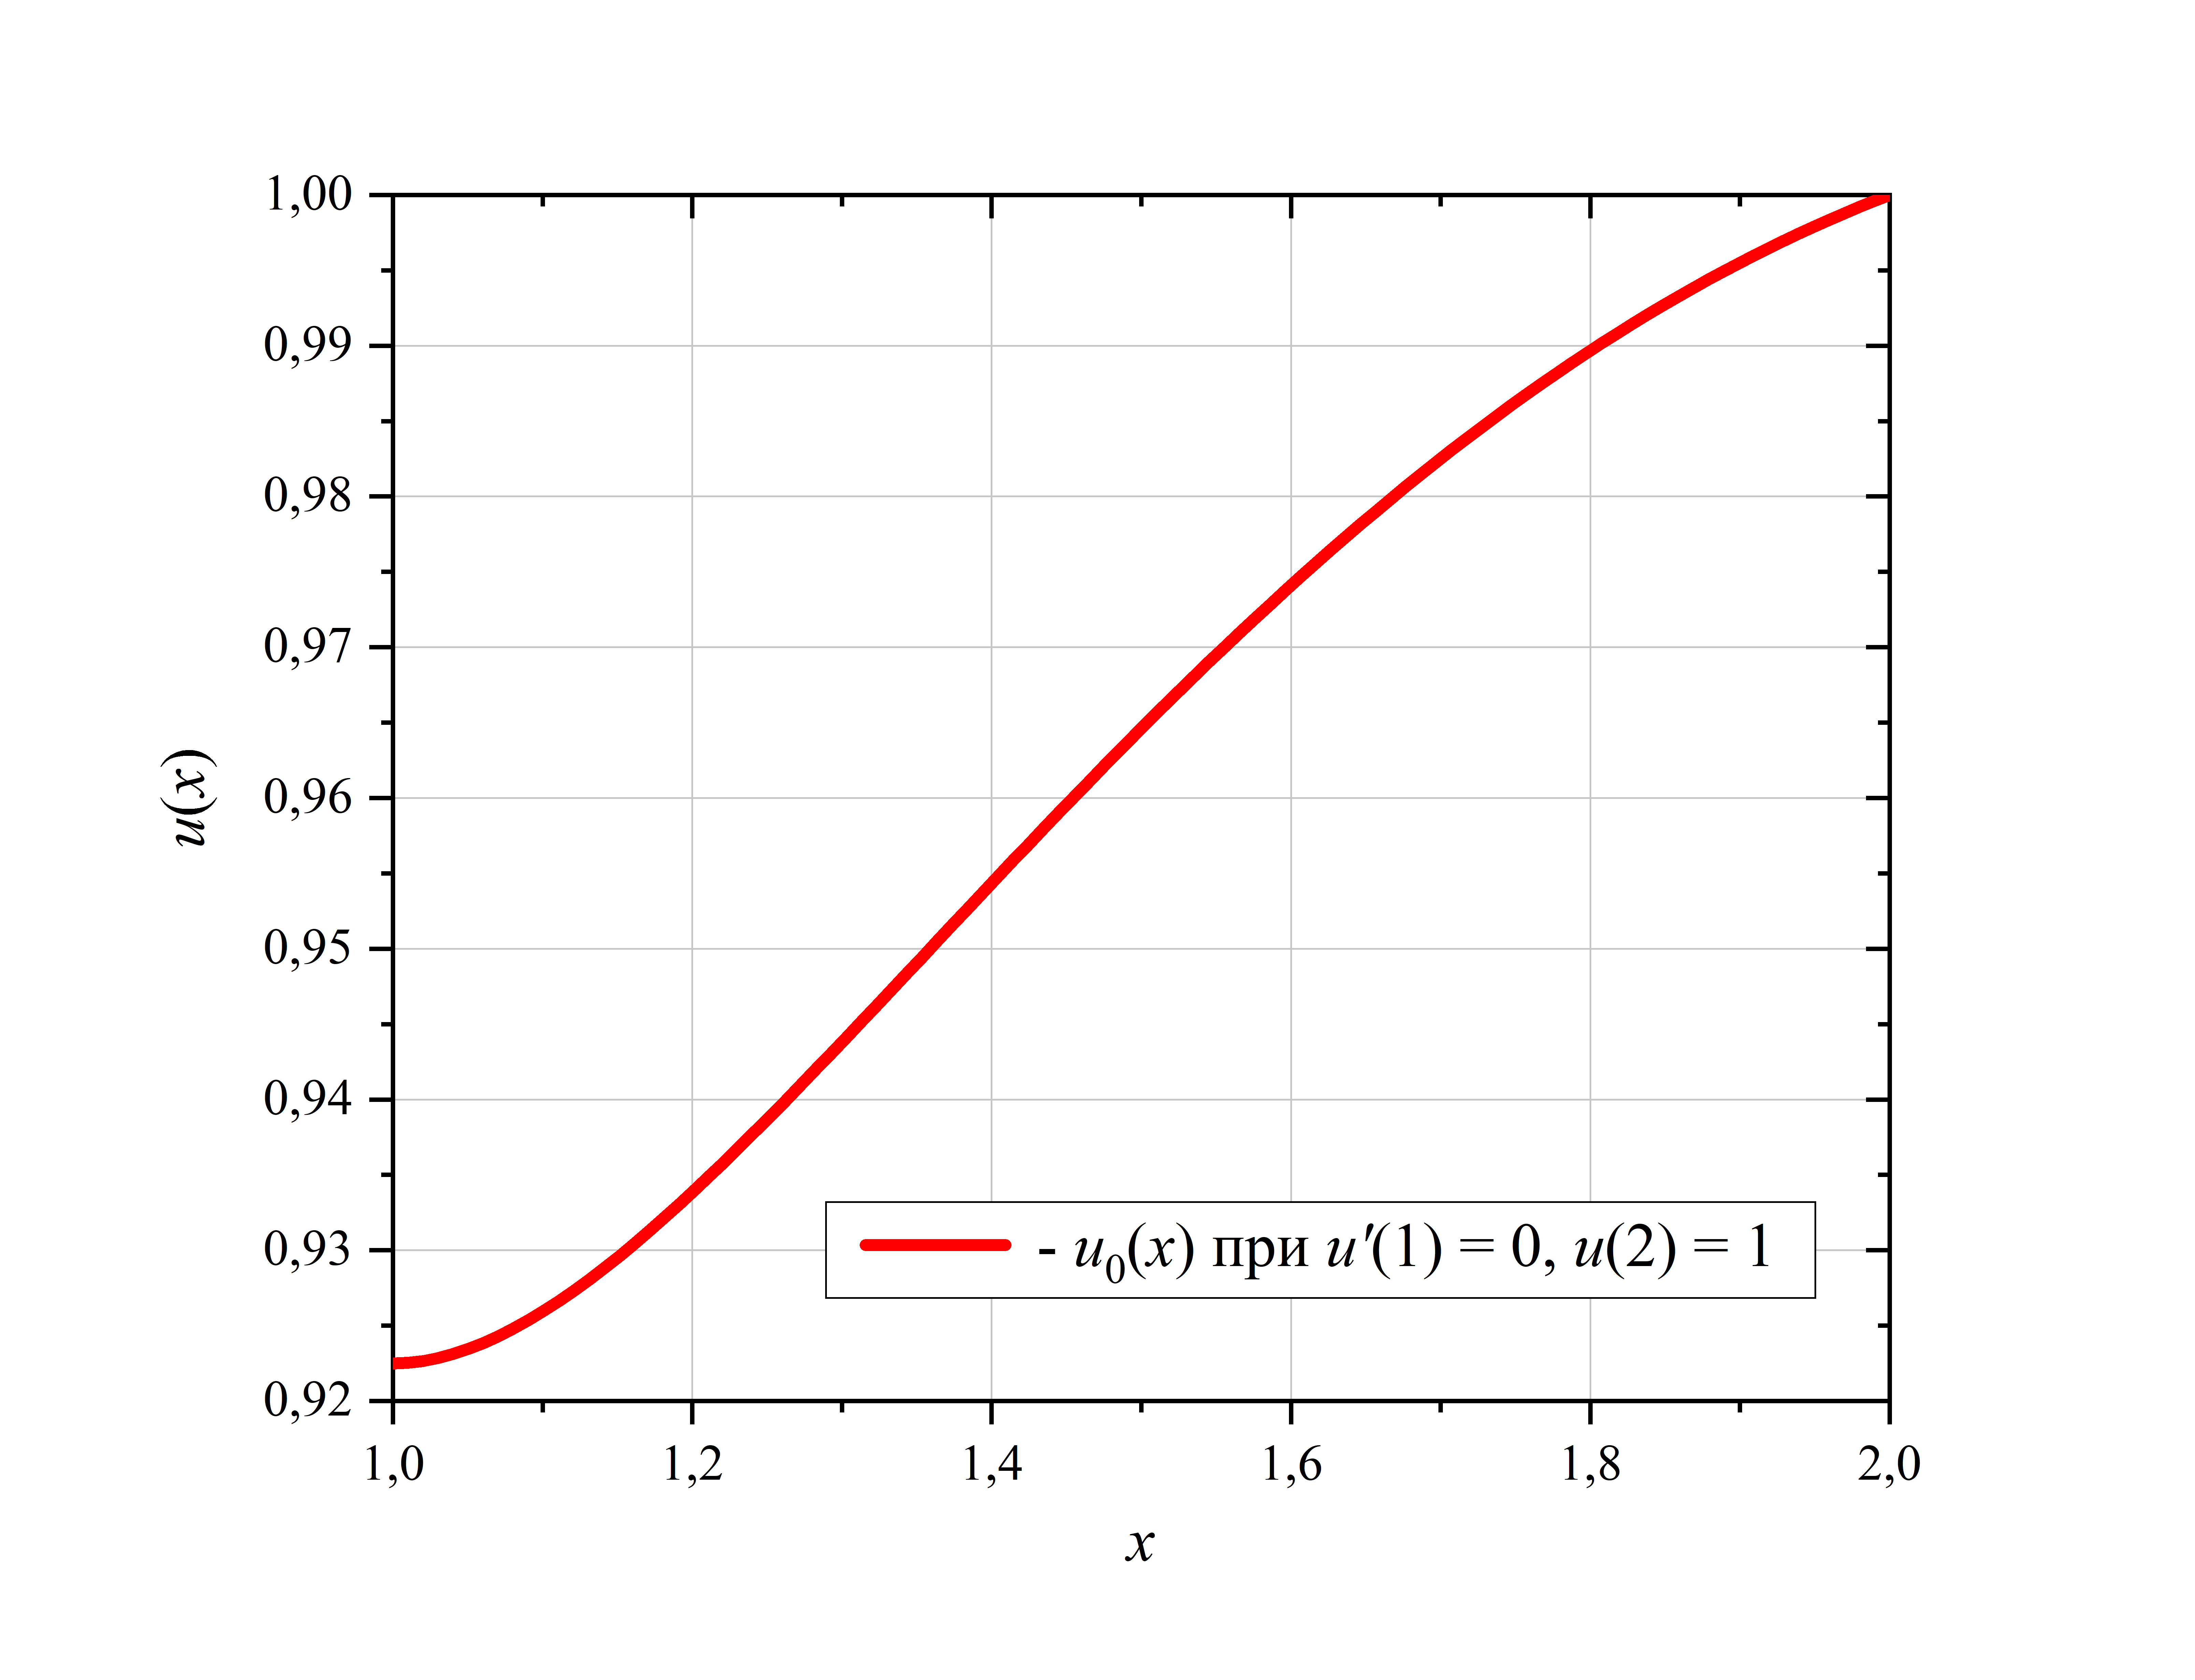
\includegraphics[height=10cm]{images/Exact_Solution_BC_1.png}}
	\caption{}
\end{figure}

\begin{figure}[h!]
	\center{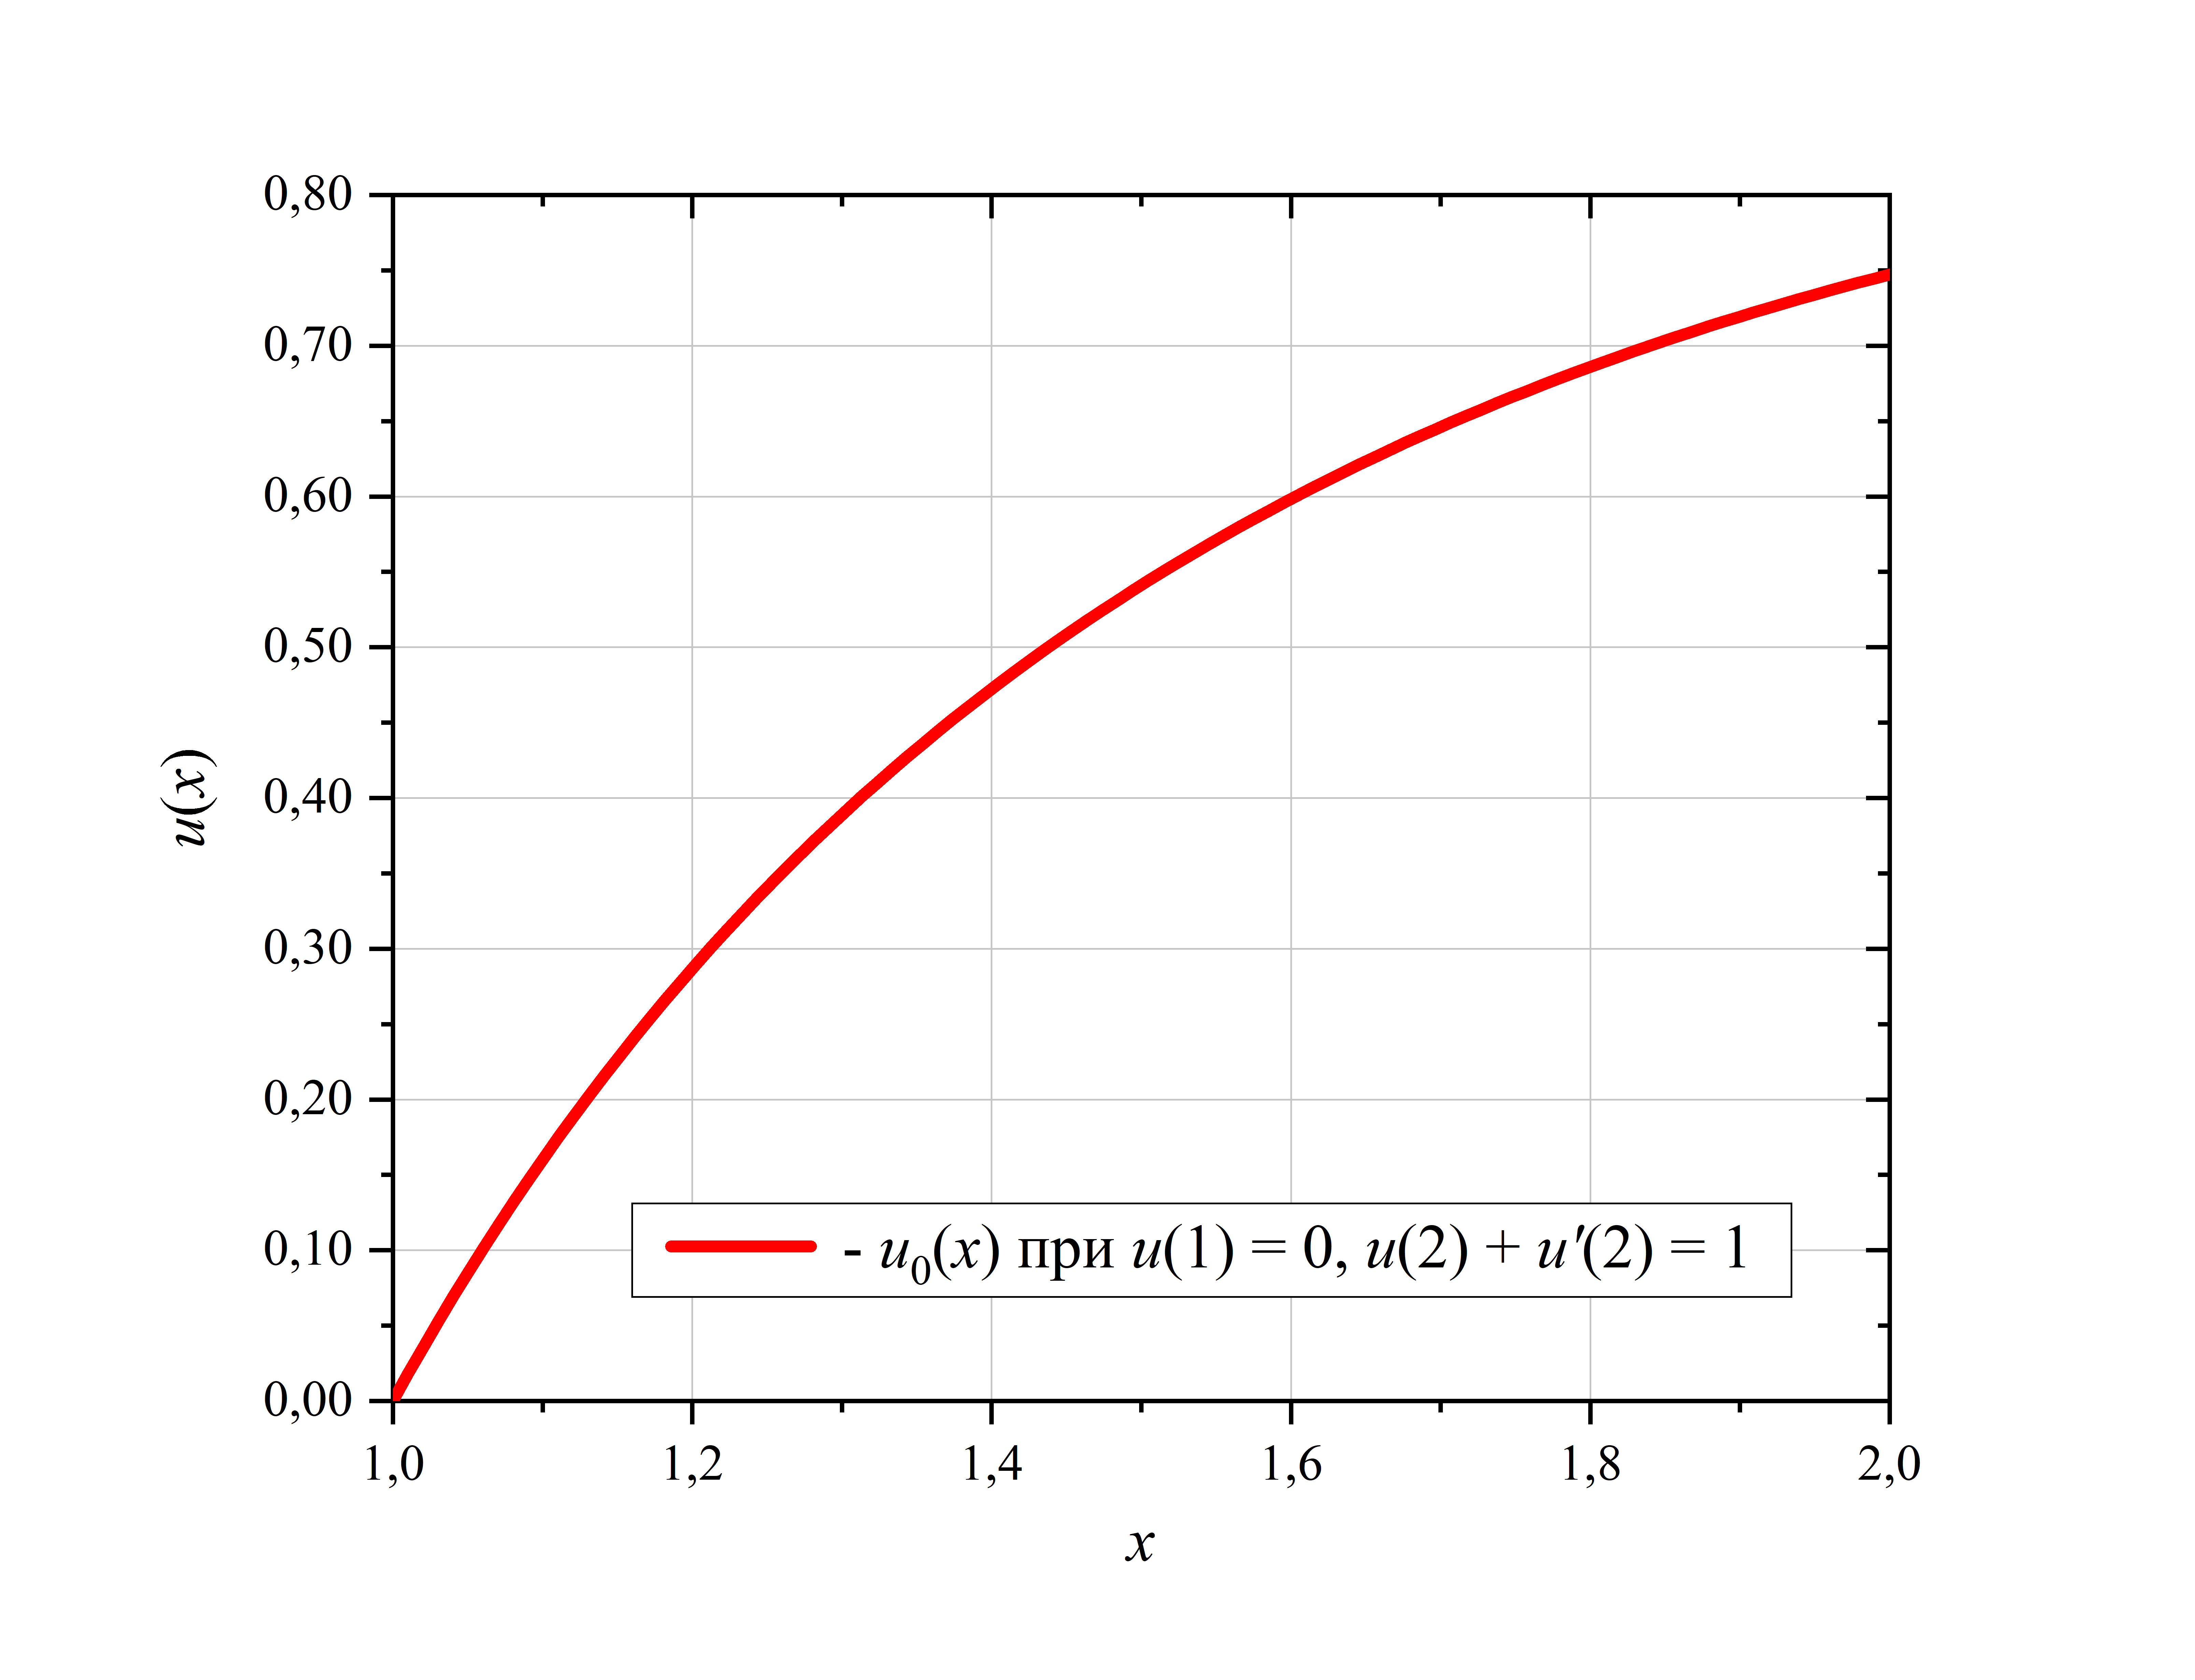
\includegraphics[height=10cm]{images/Exact_Solution_BC_2.png}}
	\caption{}
\end{figure}

\newpage
\section{}\label{appendix_b}

\begin{figure}[h!]
	\center{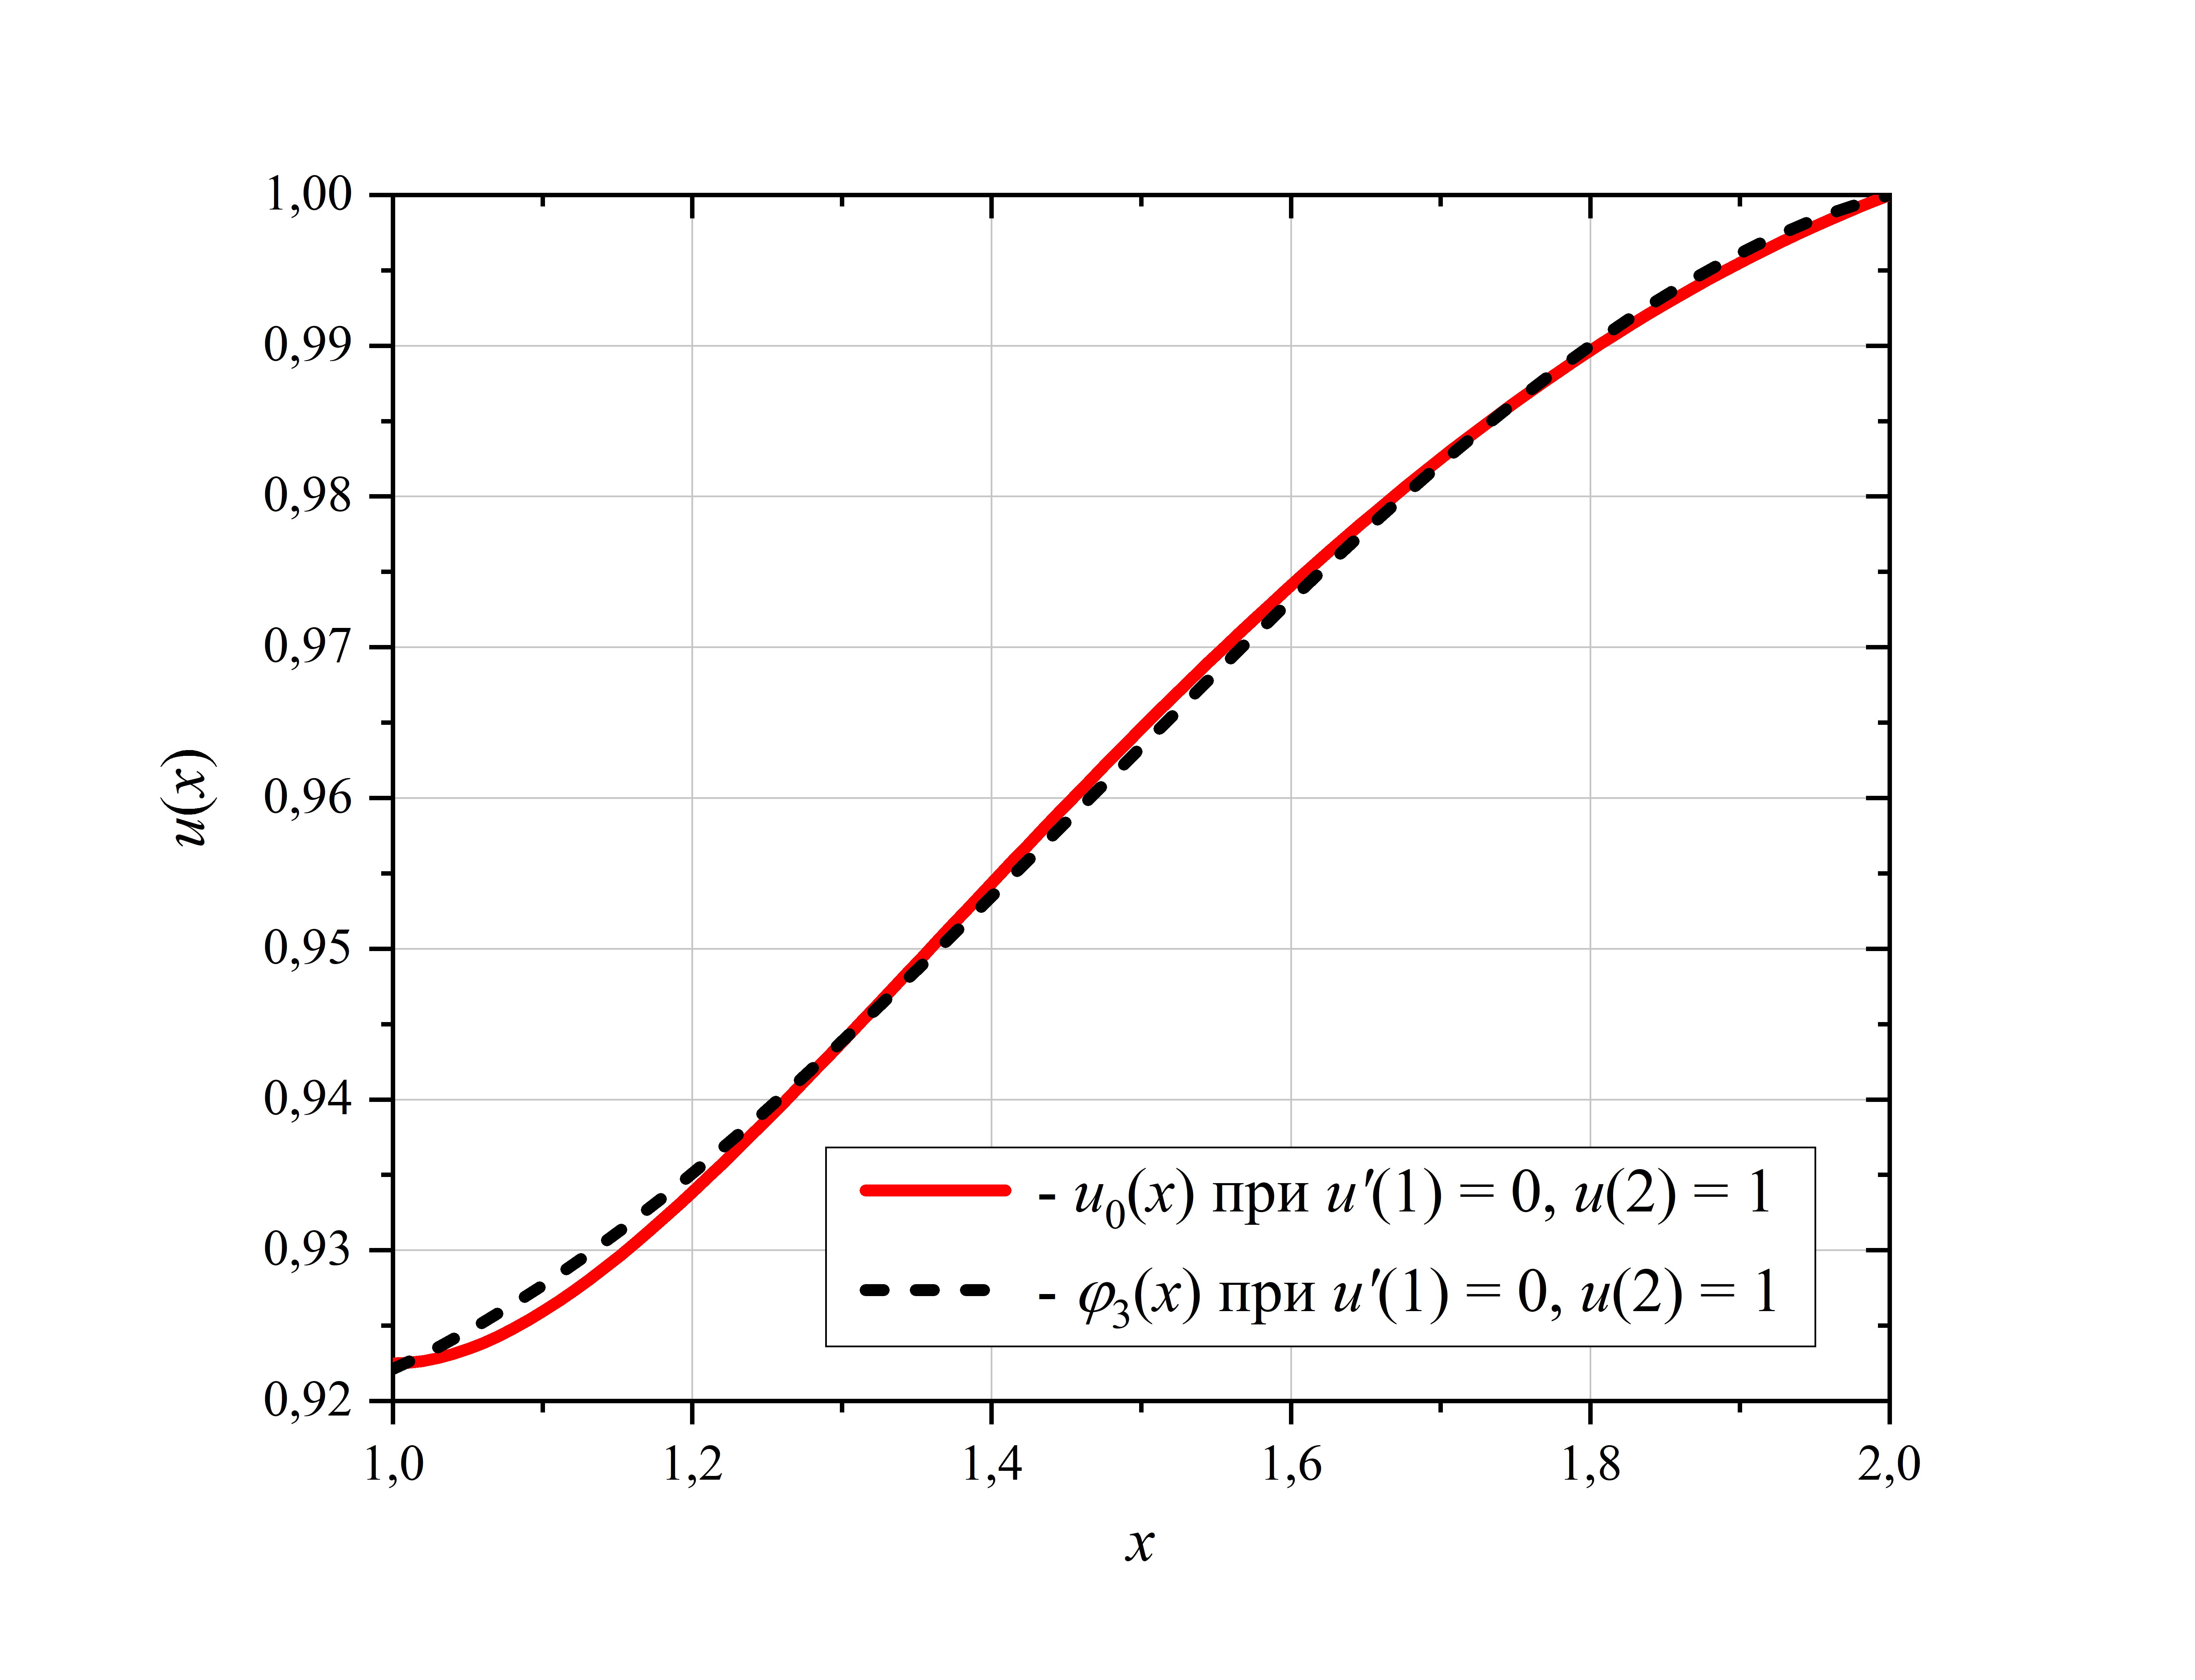
\includegraphics[height=10cm]{images/Approximate_Solution_BC_1.png}}
	\caption{}
\end{figure}

\begin{figure}[h!]
	\center{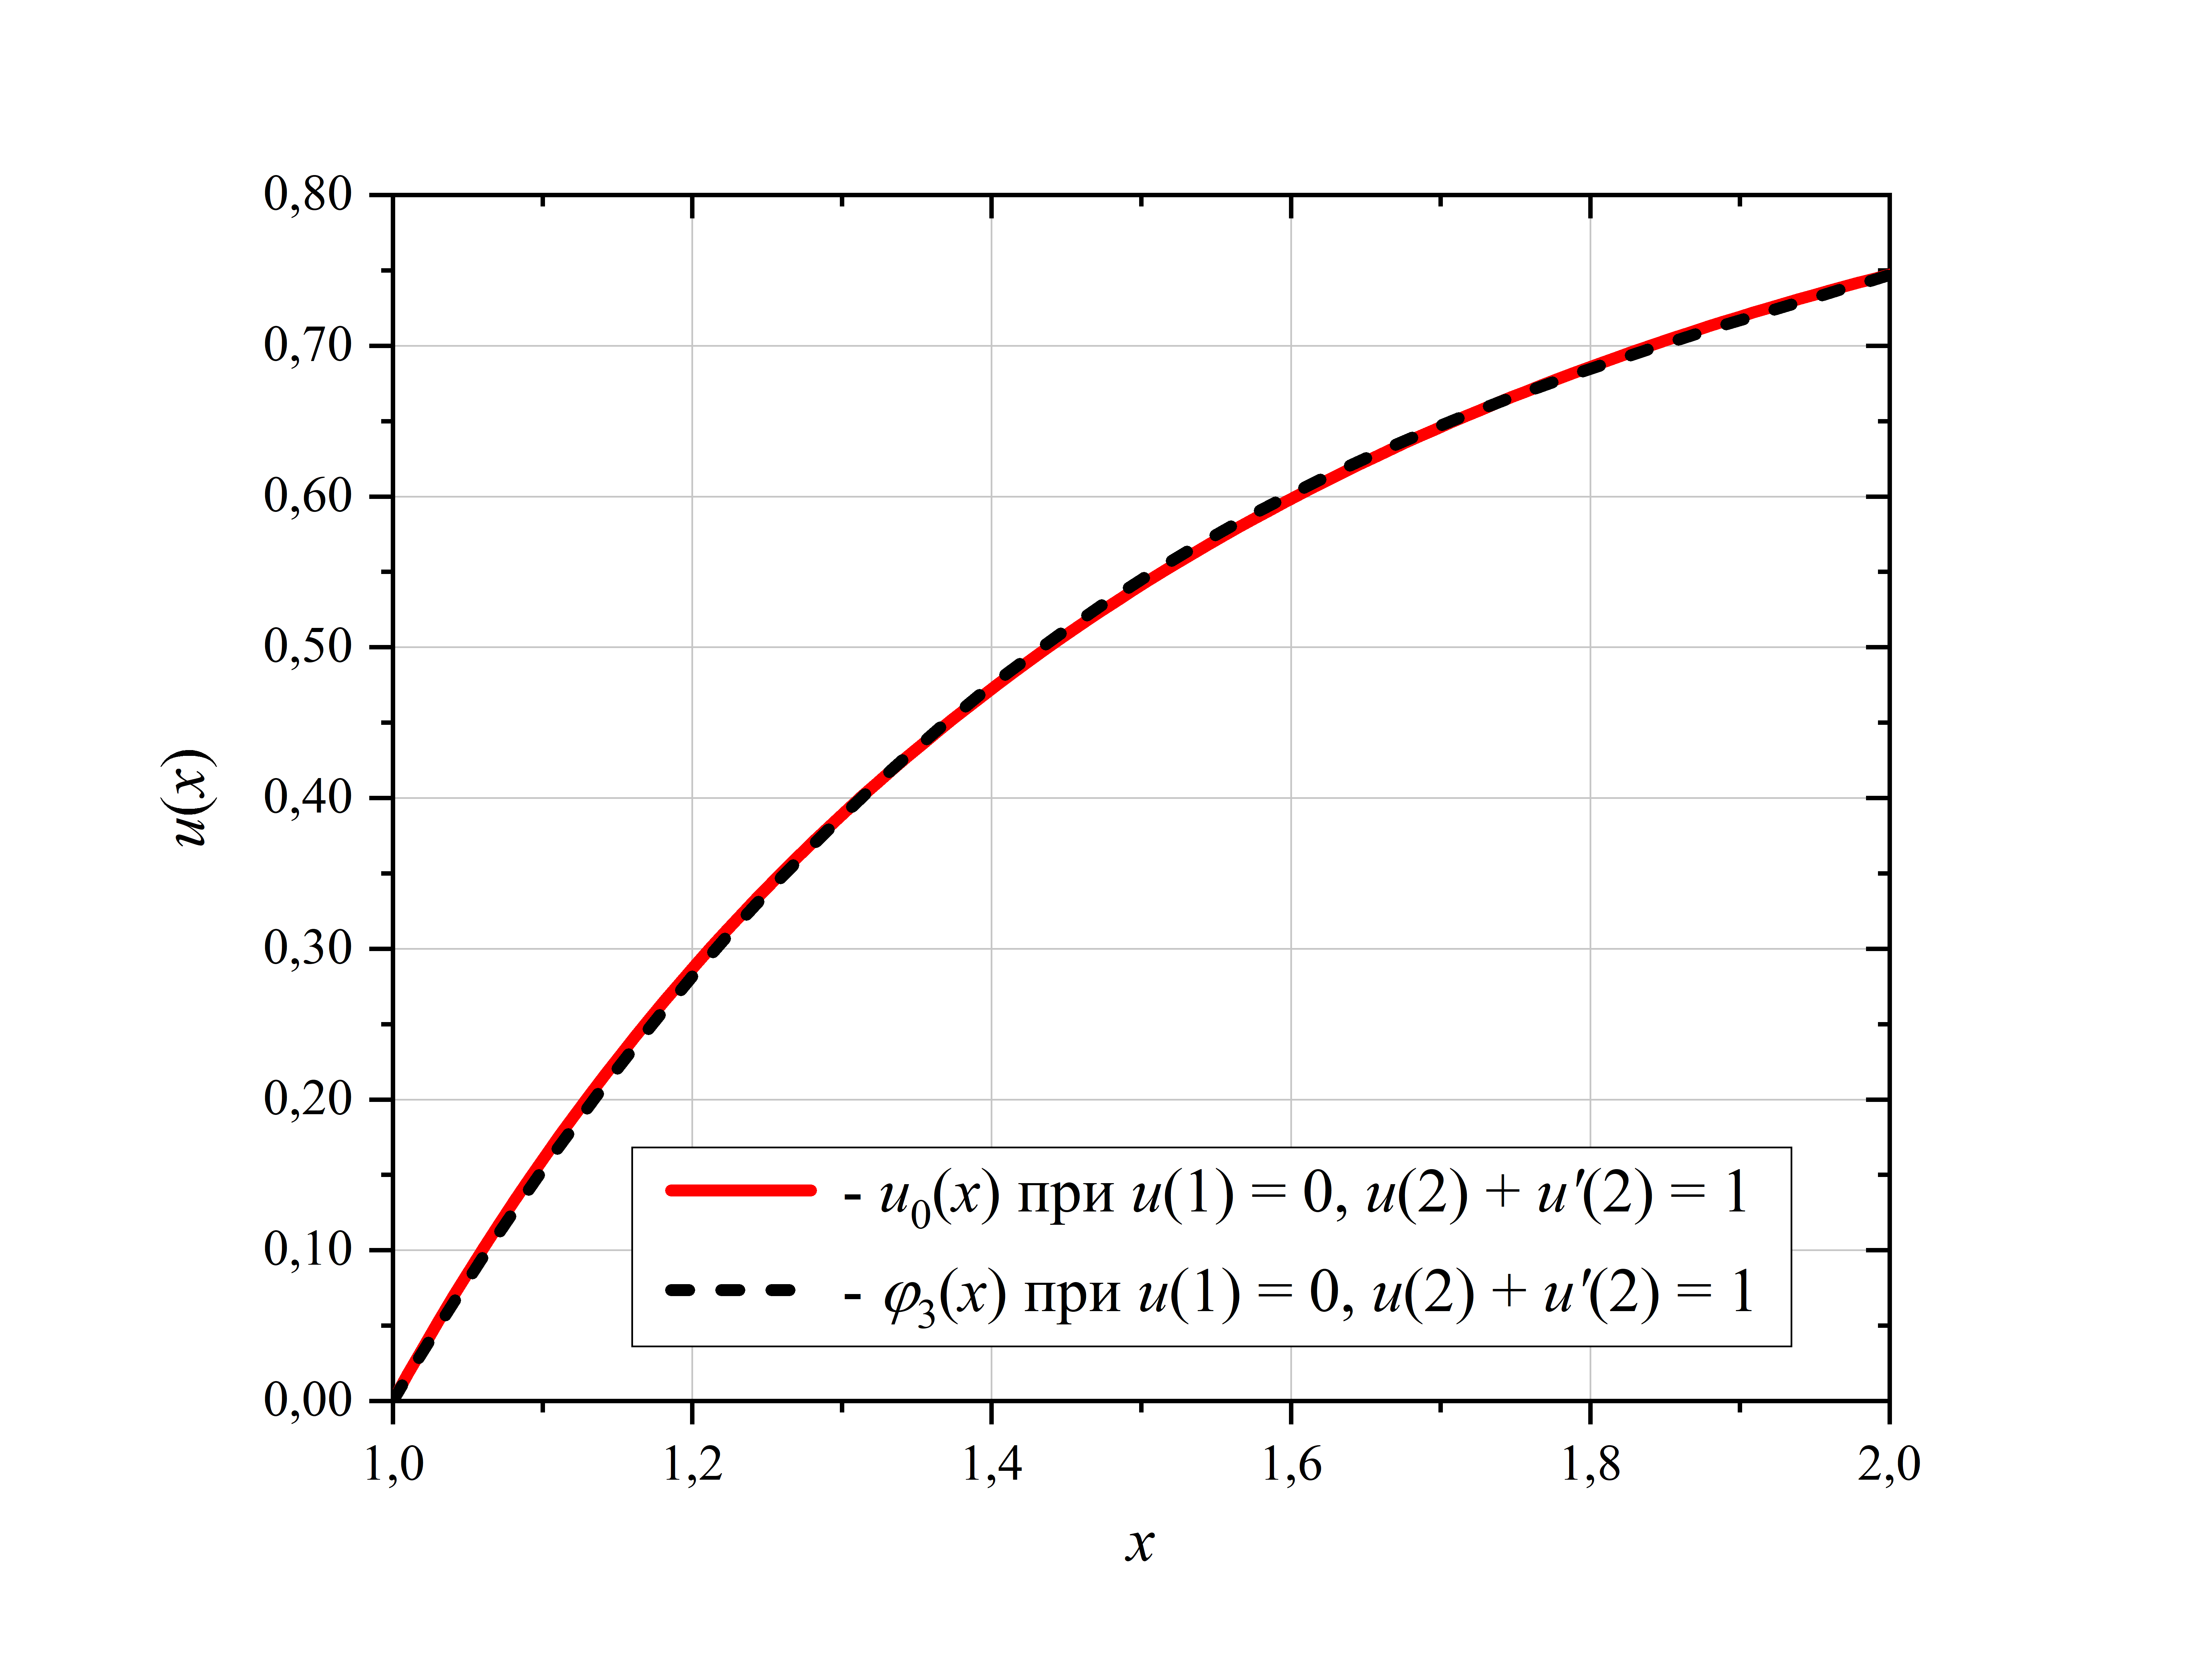
\includegraphics[height=10cm]{images/Approximate_Solution_BC_2.png}}
	\caption{}
\end{figure}

\titleformat{\section}[display]
  {\normalfont\Large\bfseries}
  {\centering Приложение\ \thesection\\}
  {0pt}{\Large\centering}
\renewcommand{\thesection}{\Asbuk{section}}

\newpage
\section{}\label{appendix_d}

\begin{warn}[ВНИМАНИЕ!]
	Вариационное исчисление способно вызвать головокружение или чрезмерную сонливость. Побочные эффекты от длительного воздействия могут включать в себя: ночную потливость, приступы паники и в редких случаях эйфорию. Прежде чем приступать к их изучению, проконсультируйтесь с врачом.
\end{warn}

\begin{question}
	Причём здесь метод конечных элементов?
\end{question}

Если мы запишем упругие смещения, вызванные приложенными нагрузками, в вариационной формулировке, мы получим

\begin{displaymath}
	u = \sum_{i=1}^n  \alpha_{i} N_{i}(x, y, z),
\end{displaymath}

\begin{displaymath}
	v = \sum_{i=1}^n  \beta_{i} M_{i}(x, y, z),
\end{displaymath}

\begin{displaymath}
	w = \sum_{i=1}^n  \gamma_{i} O_{i}(x, y, z).
\end{displaymath}

\noindent Здесь $N_{i}, M_{i}, O_{i}$ -- заранее выбранные финитные функции, а $\alpha_{i}, \beta_{i}, \gamma_{i}$ -- неизвестные коэффициенты, которые могут быть определены из условий минимума полной потенциальной энергии системы.

Главной трудностью при использовании прямых вариационных методов является выбор финитных функций $N_{i}, M_{i}, O_{i}$. 
Разумеется, что с увеличением числа финитных функций точность решения повышается, однако учёт локальных особенностей геометрии и напряжённого состояния в них (то есть уточнение концентраторов напряжений) остаётся весьма трудным.

В методе конечных элементов область поиска решения разбивается на малые конечные области. Аппроксимация функций $u, v, w$ проводится в каждой области (конечном элементе) отдельно. Этот подход позволяет принять за неизвестные смещения в узловых точках, сопрягающих отдельные области.

Подобный подход позволяет использовать простейшие финитные функции, такие как линейные или квадратичные функции координат. Далее как и в прямых вариационных методах, для получения расрешающей системы уравнений относительно неизвестных смещений узлов можно использовать начало возможных перемещений:

\begin{displaymath}
	\iiint\limits_V \{ \delta \varepsilon \}^{T} \{\sigma\} \,dV - \iiint\limits_V \{ \delta u \}^{T} \{ F \} \,dV - \iint\limits_S \{ \delta u \}^{T} \{ p \} \,dS = 0.
\end{displaymath}

С точки зрения вычислительной математики, идея метода конечных элементов заключается в том, что минимизация функционала для вариационной задачи производится на наборе простых финитных функций, каждая из которых определена в локальных подобластях. Если использовать более грубую формализацию, то метод конечных элементов можно рассматривать как один из вариантов метода Ритца.

\newpage
\begin{question}
	А как быть с матрицей жёсткости в МКЭ?
\end{question}

Чтобы объяснить связь с матрицей жесткости в МКЭ обратимся к нетривиальному, но не менее интересному подходу из квантовой механики. А если быть более точным из квантовой химии.
Допустим, что у нас существует квантовая система, энергия основного состояния $E_{0}$ которой удовлетворяет неравенству.

\begin{displaymath}
	E_{0} \leq \frac{\expval{\hat{H}}{\varPsi}}{\bra{\varPsi} \ket{\varPsi}},
\end{displaymath}

\noindent где $\varPsi$ -- неизвестная волновая функция, а $\hat{H}$ -- гамильтониан.

Применяя анзац-подход из теоретической физики сделаем предположение, 
что решение имеет специфическую форму этой волновой функции, например многочлен или экспоненту. Введем пробную волновую функцию $\varPhi$ с рядом неопределённых параметров, 
которая довольно точно опишет искомую волновую функцию $\varPsi$. Так как функция аппроксимации в методе Ритца представляет собой линейную комбинацию из $m$ известных финитных функций $\{ N_{i} \}$, параметризованную неизвестными коэффициентами $\alpha_{i}$, можем записать

\begin{displaymath}
	\varPhi = \sum_{i=1}^{m} \alpha_{i} N_{i}.
\end{displaymath}

Учитывая неравенство выше пробная волновая функция $\varPhi$ всегда будет давать математическое ожидание больше или равное основной энергии.

Имея известный гамильтониан $\hat{H}$, можно записать его математическое ожидание в виде

\begin{displaymath}
	E = \frac{\expval{\hat{H}}{\sum_{i=1}^{m} \alpha_{i} N_{i}}}{\bra{\sum_{i=1}^{m} \alpha_{i} N_{i}} \ket{\sum_{i=1}^{m} \alpha_{i} N_{i}} } = 
	\frac{\sum_{i=1}^{m} \sum_{j=1}^{m} \alpha_{i}^{*} \alpha_{j} H_{ij}}{\sum_{i=1}^{m} \sum_{j=1}^{m} \alpha_{i}^{*} \alpha_{j} S_{ij}} \equiv 
	\frac{A}{B}.
\end{displaymath}

Финитные функции обычно не ортогональны, поэтому квадратная матрица перекрытия $S_{ij}$ будет иметь ненулевые недиагональные элементы. 
Либо набор $\{ \alpha_{i} \}$, либо $\{ \alpha_{i}^{*} \}$ можно использовать для минимизации математического ожидания.

Например, для любого $k = 1, 2, \dots, m$ частная производная $\partial E / \partial \alpha_{k}^{*}$ становится равенством

\begin{displaymath}
	\frac{\partial E}{\partial \alpha_{k}^{*}} = \frac{\sum_{j=1}^{m} \alpha_{j} (H_{kj} - E S_{kj})}{B}= 0,
\end{displaymath}

\noindent которое приводит к системе из $m$ характеристических уравнений

\begin{displaymath}
	\sum_{j=1}^{m} \alpha_{j} (H_{kj} - E S_{kj}) = 0,
\end{displaymath}

\noindent для каждого $k$. Здесь $E$ - энергия, $\{ \alpha_{j} \}$ -- неизвестные коэффициенты.

На языке метода конечных элементов матрица $H_{kj}$ в точности является матрицей жёсткости гамельтониана $\hat{H}$ в кусочно-линейном пространстве элементов.
Матрица $S_{kj}$ -- матрица масс. На языке линейной алгебры значение $E$ -- собственное значение дискретизированного гамельтониана, а набор $\{ \alpha_{j} \}$  формирует дискретизированный собственный вектор.

\begin{info} % Information block
	Используемая в квантовой химии матрица перекрытия $S_{ij}$ используется для описания взаимосвязи набора базисных векторов квантовой системы.
\end{info}

\newpage
\begin{question}
	Я очень хочу решить какое-нибудь обыкновенное дифференциальное уравнение методом Ритца, но у меня не хватает математической подготовки. Как мне быть?
\end{question}

Рекомендую воспользоваться любой системой компьютерной математики, например Maplesoft Maple. Попробуем решить краевую задачу методом Ритца для уравнения

\begin{displaymath}
	\frac{d}{dx} \left( x^{2} \frac{du}{dx} \right) - 2u = -1 - \frac{2}{x}; \; \; \; u(1) = 0, \; u'(2) = 1.
\end{displaymath}

Сначала найдем эквивалентную вариационную формулировку данной задачи. Сравнивая уравнение (\ref{ODE_rank_2}) с нашим уравнением, получаем, что $p(x) = x^{2}$, $q(x) = 2$, $f(x) = 1 + 2/x$. Аналогично из вида граничного условия $u'(2) + \xi_{2} u(2) = \eta_{2}$ находим $\xi_{2} = 0$, $\eta_{2} = 1$. Граничное условие при $x = 1$ (1-го рода) является главным. Таким образом, можем построить функционал

\begin{displaymath}
	\Phi[u] = \frac{1}{2} \int_{1}^{2} \left[ x^{2} u'^{2} + 2 u^{2} - 2 \left( 1 + \frac{2}{x} \right) u \right] dx - 4 u(2).
\end{displaymath}

Выберем аппроксимирующие функции. Они должны быть такими, чтобы при любых значениях парамет-
ров $\{\alpha_{i}\}$ удовлетворяли главному граничному условию $u(1) = 0$:

\begin{displaymath}
	\varphi_{n}(x) = (\alpha_{1} + \alpha_{2}x + \alpha_{3}x^{2} + \dots + \alpha_{n}x^{n-1}) (x-1).
\end{displaymath}

Определив условия и требования, решим задачу с помощью системы компьютерной математики.

\begin{commandline}
	\begin{verbatim}
		# 1. Очистка ОЗУ
		restart;		
		
		# 2. Возьмём четыре параметра аппроксимации, положим n = 4
		phi_n := x -> ((a1 + a2*x + a3*x^2 + a4*x^3) * (1 - x));	
		
		# 3. Вычислим функционал от этой функции
		F := phi_n -> (1/2.)*int(x^2 * diff(phi_n(x), x)^2 + 2*phi_n(x)^2
		- 2*(1 + 2*1/x)*phi_n(x), x = 1..2) - 4*phi_n(2);
		
		# 4. Формируем функцию многих переменных, превращая в неё функционал
		P := F(phi_n);	
		
		# 5. Производим поиск минимума функционала, как функции многих переменных.
		#    Формируем систему алгебраических уравнений из условия экстремума dF/dai = 0
		eqSys := {diff(P, a1) = 0, diff(P, a2) = 0, diff(P, a3) = 0, diff(P, a4) = 0};
		
		# 6. Решаем полученную СЛАУ
		rs := solve(eqSys, {a1, a2, a3, a4});
		
		# 7. Представим корни СЛАУ в числовом формате
		numRoots := evalf(rs);
		
		# 8. Оформим решение задачи в виде новой функции
		phi := unapply(subs(numRoots, phi_n(x)), x);
	\end{verbatim}
\end{commandline}

\newpage
\begin{question}
	Можно ли представить решение таблично или графически?
\end{question}

Да, конечно можно. Добавим в представленный выше код такие строки:

\begin{commandline}
	\begin{verbatim}
		# 9. Обратимся к решению функции, для получения значения в точке x = 1.25
		phi(1.25);
		
		# 10. Протабулируем эту функцию на отрезке x = [1, 2] с шагом 0.25
		for t from 1 by 0.25 to 2 do printf("x=%g phi=%g\n", t, phi(t)); od;
		
		# 11. Построим график функции
		plot(phi(x), x = 1..2);
	\end{verbatim}
\end{commandline}

\begin{warn}[ВНИМАНИЕ!]
	Важные нюансы применения системы Maple.
	
	Замечание 1. В ряде случаев Maple может некорректно выводить функционал, представляя его в виде дробно-рациональной функции относительно параметров $\{\alpha_{i}\}$, в то время как он должен быть квадратичным по ним. Подобная ситуация делает применение метода Ритца невозможным. Как правило, действие Maple-функции \textbf{\texttt{expand}} на второе слагаемое под знаком интеграла в функционале, то есть $q(x)u^{2}$, помогает устранить проблему. В частности, в рассматриваемом примере в функционале $F$ вместо \textbf{\texttt{2*phi\char`_n(x)\^{}2}} следует использовать \textbf{\texttt{evalf(2*phi\char`_n(x)\^{}2)}}.
	
	Замечание 2. Как известно, Maple, в первую очередь, стремится проводить символьные вычисления, поэтому и функционал здесь выведен в символьном виде, что не всегда бывает целесообразным. Добиться числового формата можно, как всегда, с помощью \textbf{\texttt{evalf}}. Например, вместо строки "\textbf{\texttt{P := F(phi\char`_n);}}" \; записать \; "\textbf{\texttt{P := evalf(F(phi\char`_n));}}".
	
	Замечание 3. Следует помнить, что здесь коэффициенты записаны с ограниченным числом значащих цифр. В некоторых случаях это может привести к дополнительной ошибке в решении. Уменьшить такую ошибку можно заданием фиксированного числа разрядов в переменной \textbf{\texttt{Digits}}. Другой способ -- использование переменной \textbf{\texttt{rs}} вместо \textbf{\texttt{numRoots}} в определении функции \textbf{\texttt{phi}}.
\end{warn}

\begin{question}
	Можно ли представить точное решение данного дифференциального уравнения?
\end{question}

Да, конечно можно. Добавим в представленный выше код такие строки:

\begin{commandline}
	\begin{verbatim}
		# 12. Запишем и решим ДУ
		G := dsolve({diff(x^2 * diff(y(x), x), x) - 2*y(x) = - 1 - 2*1/x,
		y(1) = 0, D(y)(2) = 1}, y(x));
		
		# 13. Получим точное решение
		u := unapply(subs(G, y(x)), x);
	\end{verbatim}
\end{commandline}

\newpage
\begin{question}
	А сравнить точное и приближенное решения?
\end{question}

Без проблем. Вновь добавим в представленный выше код такие строки:

\begin{commandline}
	\begin{verbatim}
		# 14. Сначала сравним результаты в отдельных точках 
		for t from 1 by 0.25 to 2 do printf(`x=%g phi=%g u=%g\n', t, phi(t), u(t)); od;

		# 15. Для визуального сравнения построим графики
		plot([phi(x), u(x)], x = 1..2, color = [red, blue], thickness = [2, 2]);
	\end{verbatim}
\end{commandline}

Для количественной характеристики процесса сходимости используем норму ошибки решения

\begin{displaymath}
	\delta = \sqrt{ \int_{a}^{b} \left[ \varphi_{n}(x) - u(x) \right]^{2} dx },
\end{displaymath}

\noindent здесь $\varphi_{n}(x)$ -- приближенное решение методом Ритца, а $u(x)$ -- точное решение. Если метод сходится, то $\delta$ приближается к нулю с увеличением $n$ -- степени аппроксимационного полинома. То, насколько быстро это происходит, характеризует скорость сходимости.

Организуем вычисление нормы ошибки следующим образом:

\begin{commandline}
	\begin{verbatim}
		# 16. Проверим сходимость
		evalf(int((phi(x) - u(x))^2, x = 1..2))^(1/2);
	\end{verbatim}
\end{commandline}

\noindent Кроме того, можно оценить сходимость производной $\varphi_{n}'(2)$ к точному значению $1$ для граничного условия.

\begin{commandline}
	\begin{verbatim}
		# 17. Оценим сходимость первой производной
		D(phi)(2);

		# 18. Значение функционала для приближенного решения
		F(phi);

		# 19. Значение функционала для точного решения
		evalf(F(u))
	\end{verbatim}
\end{commandline}

\noindent Предлагаю, вам оценить сходимость решения для $n = 2, 3, 5, 6$. Результаты будут свидетельствовать о высокой скорости сходимости метода Ритца.

\newpage
\begin{question}
	Что не так с методом Рэлея-Ритца? Почему это разные методы?
\end{question}

\begin{warn}[Важно!]
	К сожалению, метод Ритца очень часто путают с методом Рэлея-Ритца. Название "метод Рэлея-Ритца"\;(в контексте одного из прямых методов вариационного исчисления) является распространённым неправильным термином. Метод Рэлея-Ритца -- это численный метод поиска приближенных решений уравнений на собственные значения, которые сложно решить аналитически. Он особенно актуален в контексте решения физических краевых задач, которые могут быть выражены в виде матричных дифференциальных уравнений. Он используется в машиностроении для аппроксимации собственных мод физической системы, например для нахождения резонансных частот конструкции, что позволяет создать соответствующее демпфирование. Этот метод был изобретён Вальтером Ритцем в 1909 году, поэтому (по причине некоторого сходства) сохраняется неправильное употребление названия.
\end{warn}

Часто, метод Ритца могжет быть с упехом применим к задачам на нахождение собственных функций и собственных значений. Постараюсь объяснить на примере. Рассмотрим дифференциальное уравнение

\begin{displaymath}
	- \frac{d}{dx} \left( p(x) \frac{du}{dx} \right) + q(x)u = \lambda u,
\end{displaymath}

\noindent где $p(x) \geq 0$ имеет непрерывную производную, $q(x)$ -- непрерывна при условиях

\begin{displaymath}
	u(a) = 0, \; u(b) = 0.
\end{displaymath}

Внимательный читатель заметил, что совокупность данного уравнения и граничных условий называют краевой задачей Штурма--Лиувилля. Для любого $\lambda$ она всегда имеет нулевое решение.

\begin{info}
	Нулевое решение $u \equiv 0$ называют тривиальным.
\end{info}

Те значения параметра $\lambda$, при которых краевая задача имеет нетривиальные решения $u(x) \neq 0$, называются собственными значениями (числами), а сами решения -- собственными функциями данной задачи Штурма--Лиувилля.

\begin{info}
	Собственные функции и собственные значения обладают рядом важных свойств, среди которых необходимо отметить ортогональность любых двух собственных функций $u_{i}(x)$ и $u_{j}(x)$, отвечающих двум различным собственным числам $\lambda_{i}$ и $\lambda_{j}$:
	\begin{displaymath}
		\int_{a}^{b} u_{i}(x) u_{j}(x) dx = 0, \; i \neq j.
	\end{displaymath}
\end{info}

Можно показать, что краевая задача Штурма-Лиувилля эквивалентна следующей вариационной задаче на условный экстремум (задаче поиска минимума функционала)

\begin{displaymath}
	\Phi[u] = \int_{a}^{b} \left( p(x)u'^{2} + q(x)u^{2} \right) dx,
\end{displaymath}

\noindent при граничных условиях и изопараметрическом условии

\begin{displaymath}
	u(a) = 0, \; u(b) = 0; \; \; \int_{a}^{b} u^{2}(x)dx = 1.
\end{displaymath}

Последнее условие обеспечивает отличие от тождественного нуля решения $u(x)$, а также его нормировку. Поскольку решение изопериметрической задачи сводится к безусловной минимизации функционала

\begin{displaymath}
	\Phi[u] = \int_{a}^{b} \Lagr(x) dx, 
\end{displaymath}

\noindent где $\Lagr(x) = p(x)u'^{2} + q(x)u^{2} - \lambda u^{2}$ -- функция Лагранжа, то процедура метода Ритца переносится сюда почти естественным образом. Следует учесть, что минимизируя функционал по параметрам аппроксимации $\{\alpha_{i}\}$ с учетом изопараметрического условия мы получим нелинейную систему алгебраических уравнений относительно $\{\alpha_{1}, \dots, \alpha_{k}, \lambda\}$. Поэтому точное решение данной нелинейной системы алгебраических уравнений может быть затруднительным. Но если отказаться от включения в систему изопараметрического условия, придем к обычной матричной задаче на собственные числа из линейной алгебры, методы решения которой хорошо разработаны. Вычислив собственные числа $\lambda_{n}$ и соответствующие им собственные векторы $\{\alpha_{1}^{(n)}, \dots, \alpha_{k}^{(n)}\}$, найдем собственные функции

\begin{displaymath}
	\varphi_{n}(x) = \sum_{i}^{} \alpha_{i}^{(n)} N_{i}. 
\end{displaymath}

\noindent Затем приближенная функция $\varphi_{n}(x)$ нормируется с помощью изопараметрического условия.

\begin{info}
	Метод Ритца дает приближение для собственного значения с избытком. Отметим также, что задача Штурма--Лиувилля в более общей формулировке, равно как подобные задачи на собственные значения и собственные функции в двумерном или трёхмерном пространстве, также без особых усилий могут быть приближённо решены методом Ритца.
\end{info}

\begin{question}
	Как же тогда проверить сходимость аппроксимаций в случаях, когда точное решение задачи отсутствует или его получение затруднено?
\end{question}

С практической точки зрения это очень важный вопрос, поскольку прямые методы вариационного исчисления находят применение, прежде всего, для задач, не имеющих аналитического решения, а таких задач большинство.

Для оценки точности результатов, полученных методом Ритца или другими прямыми методами, обычно пользуются следующим теоретически, конечно, несовершенным, но практически достаточно надежным приёмом.

Во-первых, вычислив $\varphi_{n}(x)$ и $\varphi_{n+1}(x)$ сравнивают их между собой в нескольких точках $ x \in \left[a, b\right] $, либо по норме $ \parallel\varphi_{n+1}(x) - \varphi_{n}(x)\parallel$. Если в пределах требуемой точности $ \varepsilon $ их значения совпадают, то считают, что с требуемой точностью решение рассматриваемой вариационной задачи равно $ \varphi_{n}(x) $.

Во-вторых, если значения $\varphi_{n}(x)$ и $\varphi_{n+1}(x)$ пределах заданной точности $\varepsilon$ не совпадают, то вычисляют $\varphi_{n+2}(x)$ и также сравнивают между собой $\varphi_{n+1}(x)$ и $\varphi_{n+2}(x)$. Этот процесс продолжается до тех пор, пока значения $\varphi_{n+k}(x)$ и $\varphi_{n+k+1}(x)$ двух соседних приближений не совпадут в пределах заданной точности.

    }

\end{document}